\documentclass[12pt,oneside,letterpaper,spanish]{article}
\usepackage[T1]{fontenc}
\usepackage[utf8]{inputenc}
\usepackage[margin=2.25cm,headheight=26pt,includeheadfoot]{geometry}
\usepackage[spanish]{babel}
\usepackage{listings}
\usepackage{color}
\usepackage{titlesec}
\usepackage{titling}
\usepackage[framed, numbered]{matlab-prettifier}
\usepackage{changepage}
\usepackage{amsmath}
\usepackage{hyperref}
\usepackage{enumitem}
\usepackage{graphicx}
\usepackage{fancyhdr}
\usepackage{lastpage}
\usepackage{caption}
\usepackage{tocloft}
\usepackage{setspace}
\usepackage{multirow}
\usepackage{titling}
\usepackage{float}
\usepackage{comment}
\usepackage{booktabs}
\usepackage{indentfirst}
\usepackage{lscape}
\usepackage{booktabs,caption}
\usepackage[flushleft]{threeparttable}
\usepackage[spanish]{nomencl}
\usepackage{xcolor}
\usepackage{lipsum}
\usepackage{datetime2}
\usepackage{subcaption}
\usepackage{tcolorbox}
\usepackage{svg}
\usepackage{amsmath}

% --- Atributos generales ---
\pagestyle{fancy}
\fancyhf{}

\setlength{\parindent}{2em}
\title{TicTacker - Memoria del Proyecto} % to reference as \title, dont use \maketitle
\author{Francisco Fernández Condado}
\makeatletter\let\Title\@title\makeatother

% --- Bloques de código ---
\lstset{language=Matlab,
style=Matlab-editor,
basicstyle=\normalsize\mlttfamily,
numbers=left,
numberstyle={\scriptsize\color{black}},
numbersep=0.5cm											
}

% --- Diseños del texto ---
\newlist{steps}{enumerate}{1}
\setlist[steps, 1]{leftmargin=1.5cm,label = Step \arabic*:}
\renewcommand{\headrulewidth}{1pt}
\renewcommand{\footrulewidth}{1pt}
\renewcommand{\rmdefault}{ptm}
\hypersetup{
    hidelinks = true
}

% --- Encabezado y pie de página ---
\rhead{Francisco Fernández}
\lhead{\Title}
\setlength\headheight{16pt}
\setlength{\footskip}{50pt}
\lhead{\Title} %rightH title
\cfoot{\thepage}




% --- Documento ---

% --- Portada ---
\begin{document}
\begin{titlepage}
\begin{center}
\vspace{2cm}
%\textsc{Oregon State University}\\[1.5cm]

\includegraphics[width=0.6\textwidth]{root/bie.jpg}~\\[1cm]
\vspace{2cm}

\hrule
\vspace{.5cm}
{ \huge \bfseries TicTacker \\ \vspace{.5cm} Memoria del Proyecto}
\vspace{.5cm}

\hrule
\vspace{1.5cm}


\Large Desarrollo Avanzado de Software\\
\vspace{0.5cm}
\large 4º Curso\\
\vspace{1cm}
\url{https://github.com/ffernandezco/DAS-Proyecto/}\\
\vspace{1cm}
\Large Grado en Ingeniería Informática de Gestión y Sistemas de Información\\
\vspace{1cm}
\large Francisco Fernández Condado\\
\vspace{0.5cm}
\large \today\\

\end{center}
\end{titlepage}

% --- Índices ---
\newpage
\doublespacing
%\addcontentsline{toc}{section}{Índice}
\renewcommand{\baselinestretch}{1}\normalsize
\tableofcontents
\renewcommand{\baselinestretch}{1}\normalsize
%\singlespacing
\thispagestyle{fancy} % force page style

%\newpage
%\listoffigures
%\thispagestyle{fancy}

%\newpage
%\listoftables
%\thispagestyle{fancy}

\newpage

\section{Introducción} \label{ch1}
\textit{TicTacker} es una aplicación móvil para Android basada en Java + Gradle que permite ayudar a empresas y a autónomos a seguir un registro de su jornada laboral. Para ello, permite realizar un seguimiento completo de las horas y minutos trabajados cada día, permitiendo además configurar una jornada laboral con sus correspondientes horas y días laborales a fin de conocer las horas extraordinarias realizadas cada día y recibir notificaciones en caso de sobrepasar la jornada descrita. Permite a los empleados registrar su perfil para obtener una experiencia más personalizada y se sincroniza con un servidor PHP para almacenar toda la información en una base de datos MySQL remota. Es además posible personalizar su logotipo y el idioma para adaptarse a las necesidades de la empresa, así como generar ficheros CSV con los fichajes registrados que posteriormente puede importarse si así se desea o configurar recordatorios para fichar a tiempo.

\subsection{Instalación y configuración}

Para hacer uso de \textit{TikTacker}, puede utilizarse el fichero APK para realizar la instalación. Una vez instalada, será necesario autenticarse, para lo que es posible crear una nueva cuenta usando el asistente o bien utilizar el usuario de demostración haciendo uso de las siguientes credenciales:

\begin{itemize}
    \item \textbf{Usuario}: \texttt{demo}
    \item \textbf{Contraseña}: \texttt{demo}
\end{itemize}

\begin{tcolorbox}
    [colback=red!5!white,colframe=red!75!black,fonttitle=\bfseries,title=Conexión a Internet]
     Esta edición de \textit{TicTacker} realiza conexiones con el servidor de Internet \url{http://ec2-51-44-167-78.eu-west-3.compute.amazonaws.com/ffernandez032/WEB/}. Se recomienda verificar que se puede acceder a dicha dirección a través del navegador del dispositivo antes de comenzar a utilizar la aplicación.
    \end{tcolorbox}

A partir de entonces, podrán comenzar a utilizarse las funcionalidades de la aplicación.

\section{Elementos utilizados y funcionalidades} \label{ch2}
Esta aplicación es una continuación de la \href{https://github.com/ffernandezco/DAS-Proyecto}{primera versión entregada}. Para construirla, se han hecho uso de las siguientes características y elementos propios de Android, además de los detallados en la \href{https://github.com/ffernandezco/DAS-Proyecto/blob/main/doc/handout.pdf}{documentación de dicha versión}:

\begin{itemize}
    \item \textbf{Uso de una base de datos remota para el registro y la identificación de usuarios}: la base de datos anterior, además de haberse ampliado, se ha alojado en una base de datos remota a la que se accede desde ficheros PHP contenidos en el servidor \url{ec2-51-44-167-78.eu-west-3.compute.amazonaws.com}. Se permite registrar usuarios e iniciar sesión, se almacenan los fichajes, los datos de los perfiles y la configuración.
    \item \textbf{Integrar los servicios Google Maps u OpenStreetMap y Geolocalización en una actividad}: a la hora de registrar un fichaje, se almacena la ubicación en caso de estar disponible y se guarda en la base de datos. Accediendo al historial de fichajes y seleccionando uno existente, es posible ver, además de los detalles, un pequeño mapa de OpenStreetMap con \href{https://github.com/osmdroid/osmdroid}{OSMdroid} en el que se detalla la ubicación.
    \item \textbf{Uso de algún content provider para añadir, modificar o eliminar datos}: al guardar un fichaje, ahora se añade también al calendario propio del dispositivo para poder ver todos con mayor detalle. Además de añadir los eventos, en caso de no haber un calendario editable se encarga de crearlo en la cuenta de Google.
    \item \textbf{Captar imágenes desde la cámara, guardarlas en el servidor y mostrarlas en la aplicación}: en la sección de perfil, cada usuario puede elegir si tomar una foto de perfil haciendo uso de la cámara del dispositivo o si prefiere obtenerla desde la galería de imágenes del dispositivo. Para evitar los límites de PHP y saturar el servidor, las imágenes se almacenan en Base64 directamente en la base de datos, con una resolución máxima de 160x160 px. Después se muestran tanto en la vista del perfil como en el menú.
    \item \textbf{Implementación de un servicio en primer plano y gestión de mensajes broadcast durante el servicio}: al comenzar un fichaje, se registra en primer plano (\textit{Foreground}) y se muestra una notificación silenciosa persistente que se actualiza periódicamente para permitir ver el tiempo que ha pasado desde el fichaje. Deja de actualizarse al marcar la salida.
    \item \textbf{Uso de mensajería FCM}: la aplicación cuenta con la mensajería FCM de Google Firebase para permitir la recepción de notificaciones push. Se almacenan los diferentes tokens generados en la base de datos, y desde el servicio web \url{http://ec2-51-44-167-78.eu-west-3.compute.amazonaws.com/ffernandez032/WEB/notificar.php} es posible enviar una notificación a todos los usuarios\footnote{Se entiende que cada usuario tendrá únicamente un dispositivo, por lo que si se inicia sesión en un nuevo dispositivo se actualiza el token en la base de datos y, por tanto, el dispositivo anterior deja de recibir notificaciones. Se recomienda crear diferentes usuarios nuevos si se van a realizar pruebas con diferentes dispositivos.} de la aplicación.
    \item \textbf{Desarrollar un widget que tenga, al menos, un elemento que se actualice automáticamente de manera periódica}: se ha incluido un widget que permite consultar, de un vistazo, el estado del fichaje (con un botón para fichar o salir), así como las horas restantes en caso de tener un fichaje en curso.
    \item \textbf{Uso de algún servicio o tarea programada mediante alarma}: a través de la configuración, es posible habilitar un recordatorio para fichar. Este recordatorio configura una alarma y, en caso de que no se haya registrado ningún fichaje para la hora establecida, se envía una notificación programada. Para poder hacer uso de este servicio, será necesario habilitar los permisos correspondientes en la configuración del dispositivo.
\end{itemize} 

\section{Clases, estructura y bases de datos de la aplicación} \label{ch3}
\textit{TicTacker} hace uso de diferentes clases que se comunican entre sí y que utilizan los elementos XML de Android para gestionar la vista correspondiente. Adicionalmente, se hace uso de una base de datos MySQL desde un servidor con PHP para gestionar los usuarios, los fichajes, los perfiles, los tokens de FCM y las configuraciones personalizadas.

\subsection{Clases}
La aplicación cuenta con diferentes clases Java diferenciadas que dan respuesta a una o varias de las funcionalidades de la aplicación. A continuación se describen las siguientes clases utilizadas, pudiendo ver las relaciones entre las mismas por medio de diagrama de clases de la Figura \ref{fig:diagrama}.

\subsubsection{Activities}
\begin{itemize}
  \item \textbf{MainActivity}: actividad principal que se encarga de gestionar la navegación y la interfaz de usuario principal de la aplicación.
  \item \textbf{LoginActivity}: gestiona la autentificación de usuarios existentes, validando credenciales y guardando la sesión.
  \item \textbf{SignupActivity}: gestiona el registro de nuevos usuarios, incluyendo validación de los datos, que no se repitan nombres de usuario y creación de cuentas junto con un perfil básico a partir de los datos introducidos.
  \item \textbf{SettingsActivity}: ofrece opciones de personalización de la aplicación, como cambiar el idioma, la jornada laboral, el logotipo o los recordatorios de fichaje.
  \item \textbf{NoInternetActivity}: se lanza en el momento en el que se detecta que no se cuenta con conexión a Internet, bloqueando el uso de la app.
\end{itemize}

\subsubsection{Fragments}
\begin{itemize}
  \item \textbf{ClockInFragment}: fragment que permite a los usuarios registrar sus fichajes, mostrando el estado actual y el tiempo trabajado.
  \item \textbf{FichajeDetailsFragment}: permite a los usuarios ver los detalles de un fichaje concreto seleccionado del historial, dejando ver la ubicación en un mapa de OpenStreetMap en caso de estar disponible.
  \item \textbf{HistoryFragment}: fragment que muestra el historial de fichajes del usuario, permitiendo exportar e importar datos por medio de ficheros CSV.
  \item \textbf{SettingsFragment}: fragment que permite a los usuarios ajustar sus preferencias, como las horas de trabajo semanales y los días laborables.
  \item \textbf{EditFichajeDialog}: dialog fragment utilizado a la hora de editar la hora de entrada y/o salida de un fichaje existente en la aplicación.
\end{itemize}

\subsubsection{Adaptadores}
\begin{itemize}
  \item \textbf{FichajeAdapter}: utilizado para mostrar listas de fichajes a través de un \textit{RecyclerView}.
\end{itemize}

\subsubsection{Clases generales}
\begin{itemize}
  \item \textbf{TicTacker}: clase principal de la aplicación que se encarga de aplicar las preferencias de usuario al iniciar, así como de instanciar OSMdroid para poder utilizar los mapas de OpenStreetMap.
  \item \textbf{Fichaje}: entidad que representa un fichaje con los atributos correspondiente, usado para instanciar objetos fácilmente con su fecha, hora de entrada, hora de salida, latitud, longitud y nombre de usuario para almacenar en la base de datos.
  \item \textbf{WorkTimeCalculator}: clase que proporciona métodos para calcular el tiempo trabajado y el tiempo restante.
  \item \textbf{ApiClient}: clase utilizada para realizar las consultas POST y GET a la API del servidor, permitiendo realizar modificaciones sobre la base de datos.
  \item \textbf{NetworkConnectivityChecker}: clase utilizada para comprobar si se tiene conexión a Internet al ser requerida para funcionar. En caso de no tener conexión, se lanza \textit{NoInternetActivity}.
  \item \textbf{UserProfile}: clase utilizada para gestionar los perfiles de usuario, almacenando valores como el nombre, el email o la foto de perfil.
\end{itemize}

\subsubsection{Helpers}
\begin{itemize}
  \item \textbf{DatabaseHelper}: gestiona la base de datos MySQL realizando llamadas al \textit{DatabaseWorker} que, a su vez, utiliza \textit{ApiClient} para llamar a la API y hacer cambios en el servidor.
  \item \textbf{NotificationHelper}: clase que gestiona la creación y envío de notificaciones.
\end{itemize}

\subsubsection{Receivers}
\begin{itemize}
  \item \textbf{BootReceiver}: clase auxiliar utilizada para reconfigurar las alarmas de los recordatorios de fichajes en caso de que el dispositivo se reinicie.
  \item \textbf{ClockInReminderReceiver}: clase que interpreta y gestiona las alarmas enviadas por la clase \textit{ClockInReminderService} y que se encarga de generar las notificaciones de recordatorios de fichajes.
\end{itemize}

\subsubsection{Services}
\begin{itemize}
  \item \textbf{ClockInReminderService}: clase utilizada para enviar alarmas para recordar al usuario que inicie un fichaje si se supera una hora determinada y no se ha fichado.
  \item \textbf{ForegroundTimeService}: servicio empleado para gestionar la actividad de fichaje en primer plano (\textit{Foreground}), lanzando una notificación silenciosa persistente para informar del estado del fichaje.
  \item \textbf{MyFirebaseMessagingService}: servicio utilizado para registrar los tokens FCM de Firebase y recibir notificaciones enviadas a distancia.
\end{itemize}

\subsubsection{Eventos}
\begin{itemize}
  \item \textbf{FichajeEvents}: clase que gestiona los eventos relacionados con los fichajes, permitiendo notificar cambios a los listeners registrados.
\end{itemize}

\subsubsection{Widgets}
\begin{itemize}
  \item \textbf{TicTackerWidget}: clase utilizada para gestionar todos los aspectos relacionados con el widget de la aplicación.
\end{itemize}

\subsubsection{Workers}
\begin{itemize}
  \item \textbf{DatabaseWorker}: worker que envía y recibe las consultas en formato JSON realizadas a la API para realizar cambios sobre la base de datos.
  \item \textbf{WorkTimeCheckWorker}: worker que comprueba periódicamente el tiempo trabajado y envía notificaciones al usuario si alcanza su jornada laboral.
\end{itemize}

\begin{figure}[H]
    \centering
    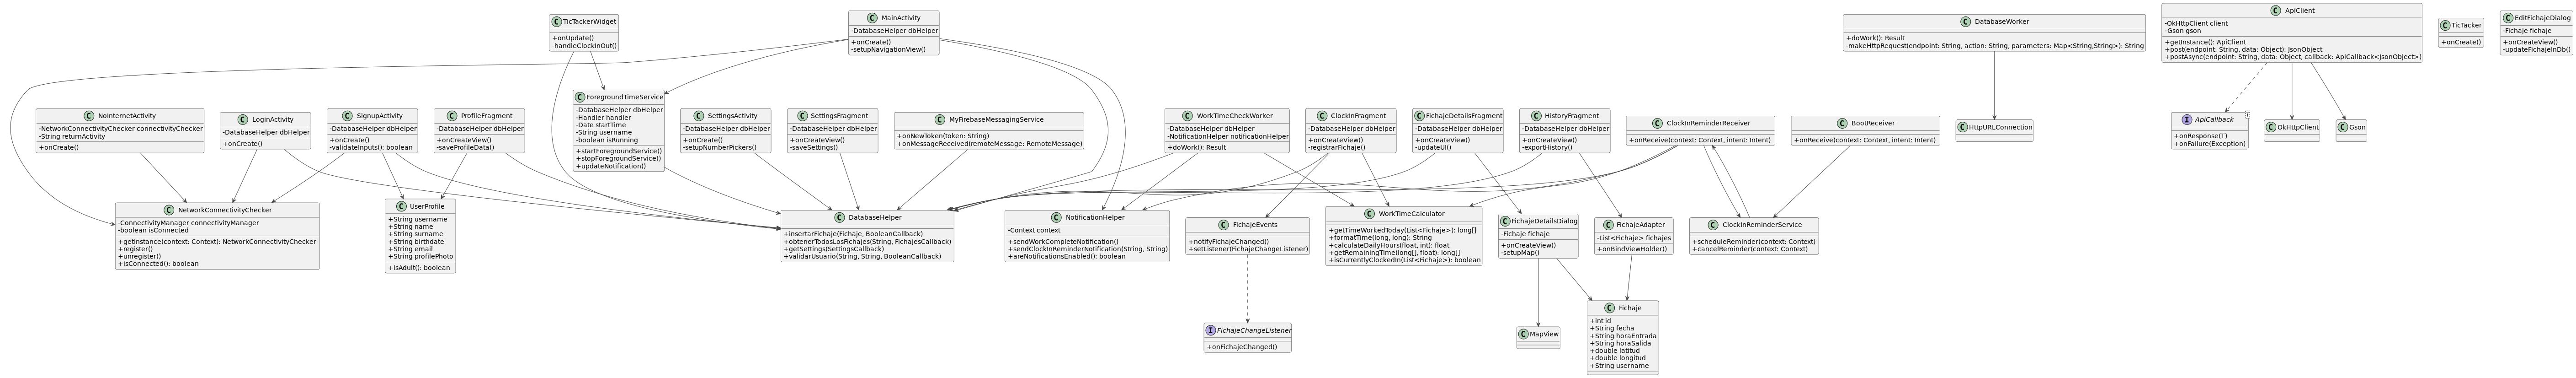
\includegraphics[width=1\linewidth]{root/diagrama.png}
    \caption{Diagrama de clases del proyecto}
    \label{fig:diagrama}
\end{figure}

\subsection{Base de datos}

Además de las \textit{SharedPreferences}, para gestionar la persistencia de la aplicación se hace uso de una base de datos de tipo MySQL controlada desde un servidor PHP, que tal y como se muestra en el diagrama de la Figura \ref{fig:bd}, contiene las siguientes tablas:

\begin{itemize}
  \item \textbf{Tabla \texttt{fichajes}}: almacena la información sobre los fichajes de los usuarios.
  \begin{itemize}
    \item \textbf{Atributos principales}: \texttt{id}, \texttt{fecha}, \texttt{hora\_entrada}, \texttt{hora\_salida}, \texttt{latitud}, \texttt{longitud}, \texttt{username}.
    \item \textbf{Índices}: \texttt{id} es un campo único y clave primaria.
  \end{itemize}
  
  \item \textbf{Tabla \texttt{users}}: almacena los usuarios registrados en la aplicación.
  \begin{itemize}
    \item \textbf{Atributos principales}: \texttt{id}, \texttt{username}, \texttt{password}.
    \item \textbf{Índices}: \texttt{username} es un campo único indexado para prevenir duplicados.
  \end{itemize}
  
  \item \textbf{Tabla \texttt{settings}}: almacena las configuraciones de horas de trabajo y recordatorios.
  \begin{itemize}
    \item \textbf{Atributos principales}: \texttt{id}, \texttt{weekly\_hours}, \texttt{working\_days}, \texttt{reminder\_enabled}, \texttt{reminder\_hour}, \texttt{reminder\_minute}.
    \item \textbf{Índices}: \texttt{id} es un campo único y clave primaria.
  \end{itemize}
  
  \item \textbf{Tabla \texttt{fcm\_tokens}}: almacena los tokens de notificaciones push para cada usuario.
  \begin{itemize}
    \item \textbf{Atributos principales}: \texttt{id}, \texttt{username}, \texttt{token}, \texttt{created\_at}, \texttt{updated\_at}.
    \item \textbf{Índices}: \texttt{id} es un campo único y clave primaria.
  \end{itemize}

  \item \textbf{Tabla \texttt{user\_profiles}}: almacena información adicional del perfil del usuario.
  \begin{itemize}
    \item \textbf{Atributos principales}: \texttt{id}, \texttt{username}, \texttt{name}, \texttt{surname}, \texttt{birthdate}, \texttt{email}, \texttt{profile\_photo}.
    \item \textbf{Índices}: \texttt{id} es un campo único y clave primaria.
  \end{itemize}
\end{itemize}

\begin{figure}[H]
    \centering
    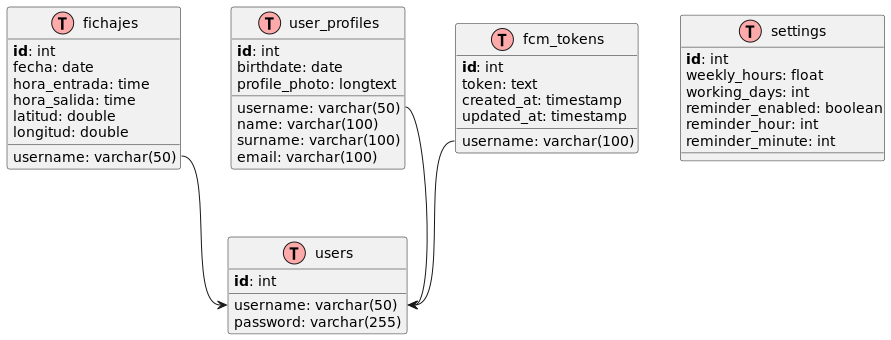
\includegraphics[width=1\linewidth]{root/bd.png}
    \caption{Diagrama de la base de datos usada del proyecto}
    \label{fig:bd}
\end{figure}

\subsection{Ficheros PHP usados en el servidor}

Para ejecutar consultas sobre la base de datos MySQL mencionada anteriormente, así como realizar los correspondientes envíos de la mensajería FCM, se han cargado a través de SFTP los siguientes ficheros en la dirección de Internet \url{http://ec2-51-44-167-78.eu-west-3.compute.amazonaws.com/ffernandez032/WEB/}, disponibles para su consulta en el \href{https://github.com/ffernandezco/TicTacker/tree/main/server}{directorio \texttt{server} del repositorio de GitHub}:

\begin{itemize}
  \item \textbf{db\_connect.php}: recoge las credenciales de conexión a la base de datos. Por motivos de seguridad, se han ocultado algunos campos en el repositorio de GitHub. Modificando los ficheros y las direcciones de la conexión es posible usar otro servidor si así se desea.
  \item \textbf{auth\_user.php}: verifica que un usuario y contraseña coinciden con el \textit{hash} almacenado en la base de datos para permitir su autenticación.
  \item \textbf{fcm\_tokens.php}: se encarga de almacenar los tokens FCM de Firebase y de actualizar si es necesario el usuario al que está asociado cada uno.
  \item \textbf{fichajes.php}: gestiona todas las operaciones relacionadas con los fichajes, incluyendo añadirlos, modificarlos o eliminarlos.
  \item \textbf{firebase\_service\_account.json}: fichero extraído del gestor de cuentas de servicio IAM de Google que contiene los datos necesarios para enviar mensajes usando la mensajería Cloud Messaging de Firebase. Por motivos de seguridad, no se ha incluido en el repositorio de GitHub.
  \item \textbf{jwt\_utils.php}: adaptación compilada del \href{https://github.com/firebase/php-jwt}{repositorio \texttt{firebase/php-jwt}} para gestionar la autenticación de Firebase desde PHP.
  \item \textbf{notificar.php}: habilita una interfaz HTML que permite enviar una notificación a todos los usuarios con un token FCM almacenado en la base de datos. Está disponible de forma pública en la dirección \url{http://ec2-51-44-167-78.eu-west-3.compute.amazonaws.com/ffernandez032/WEB/notificar.php}.
  \item \textbf{profile.php}: gestiona todas las operaciones relacionadas con los perfiles de usuario, como modificar o añadir el nombre, los apellidos, la foto de perfil o el correo electrónico.
  \item \textbf{send\_notification\_v1.php}: permite enviar notificaciones a los usuarios a través del token usando Firebase Cloud Messaging (FCM).
  \item \textbf{settings.php}: gestiona todas las operaciones relacionadas con las configuraciones, como la configuración de la jornada o el envío de notificaciones.
  \item \textbf{users.php}: gestiona todas las operaciones relacionadas con los usuarios, como añadir un usuario o modificar la contraseña asociada.
\end{itemize}

\section{Manual de usuario de TicTacker} \label{ch4}
Una vez se ha realizado la instalación de la aplicación por medio del fichero APK, será posible comenzar a utilizarla. Es necesario contar con una conexión a Internet para poder usar la misma. Al lanzarla por primera vez, en función de la versión del sistema operativo Android, se lanzarán alertas para conceder permisos de cara al envío de notificaciones, la ubicación y la gestión de archivos de imagen. Es recomendable habilitar todos ellos mientras la app esté en uso para evitar problemas de funcionamiento y aprovechar todas las características.

\subsection{Inicio de sesión y registro de usuarios}

Tras aceptar los permisos, se mostrará la pantalla de inicio de sesión representada en la Figura \ref{fig:login}. Es posible hacer uso de la cuenta de demostración, usando “\texttt{demo}” como usuario y contraseña, si bien también puede pulsarse sobre el enlace de registro para dar de alta un nuevo usuario, como representa la Figura \ref{fig:signup}. En caso de elegir esta opción, deberá indicarse un nombre de usuario que no puede existir ya en la base de datos, así como una contraseña con 4 o más caracteres que, por motivos de seguridad, deberá introducirse dos veces. También será necesario introducir el nombre, un correo electrónico válido y la fecha de nacimiento, que debe ser superior a los 18 años.

La pantalla de bienvenida de la Figura \ref{fig:fichado} ilustra una situación de fichaje en curso. La navegación por medio de los distintos apartados de la aplicación se realiza presionando sobre el botón de las tres líneas que se muestra en la esquina superior izquierda. La aplicación presenta tres áreas separadas sobre las que se darán más detalles a continuación:

\begin{itemize}
    \item \textbf{Fichar}: permite consultar el estado de un fichaje en curso o fichar a medida.
    \item \textbf{Historial}: ofrece información sobre los fichajes almacenados, además de permitir exportar e importar datos.
    \item \textbf{Ajustes}: permite definir aspectos de configuración a nivel de la aplicación. Para obtener la mejor experiencia de usuario, se recomienda comenzar accediendo a esta sección.
\end{itemize}

\begin{figure}[H]
     \centering
     \begin{subfigure}[b]{0.3\textwidth}
         \centering
         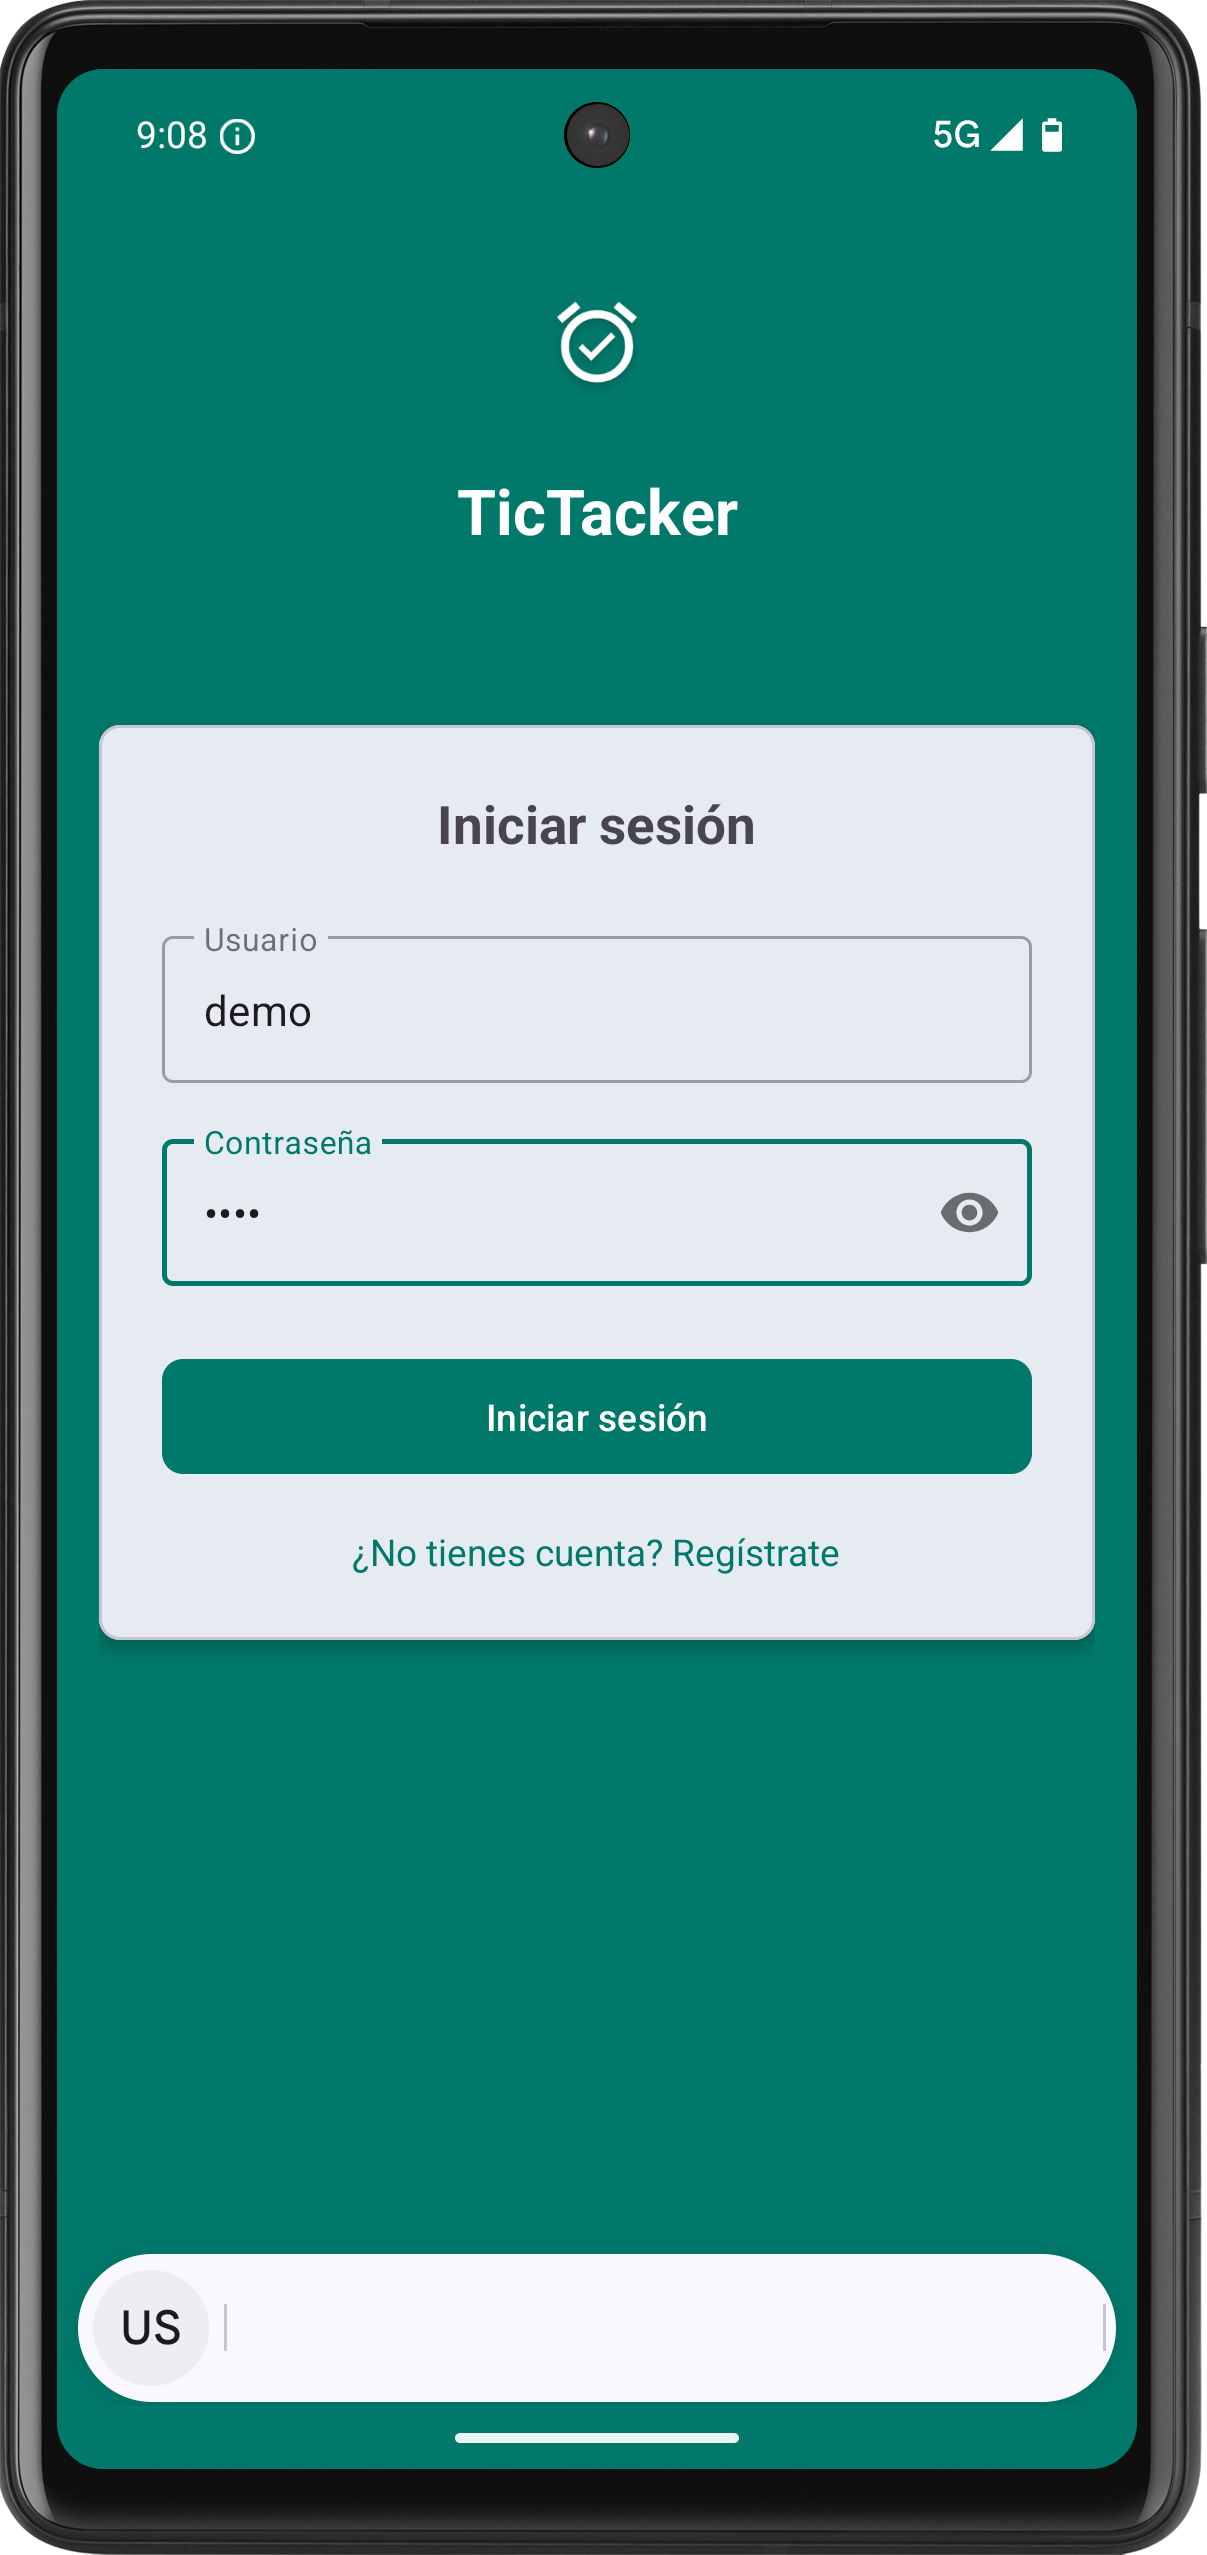
\includegraphics[width=\textwidth]{root/login.png}
         \caption{Inicio de sesión}
         \label{fig:login}
     \end{subfigure}
     \hfill
     \begin{subfigure}[b]{0.3\textwidth}
         \centering
         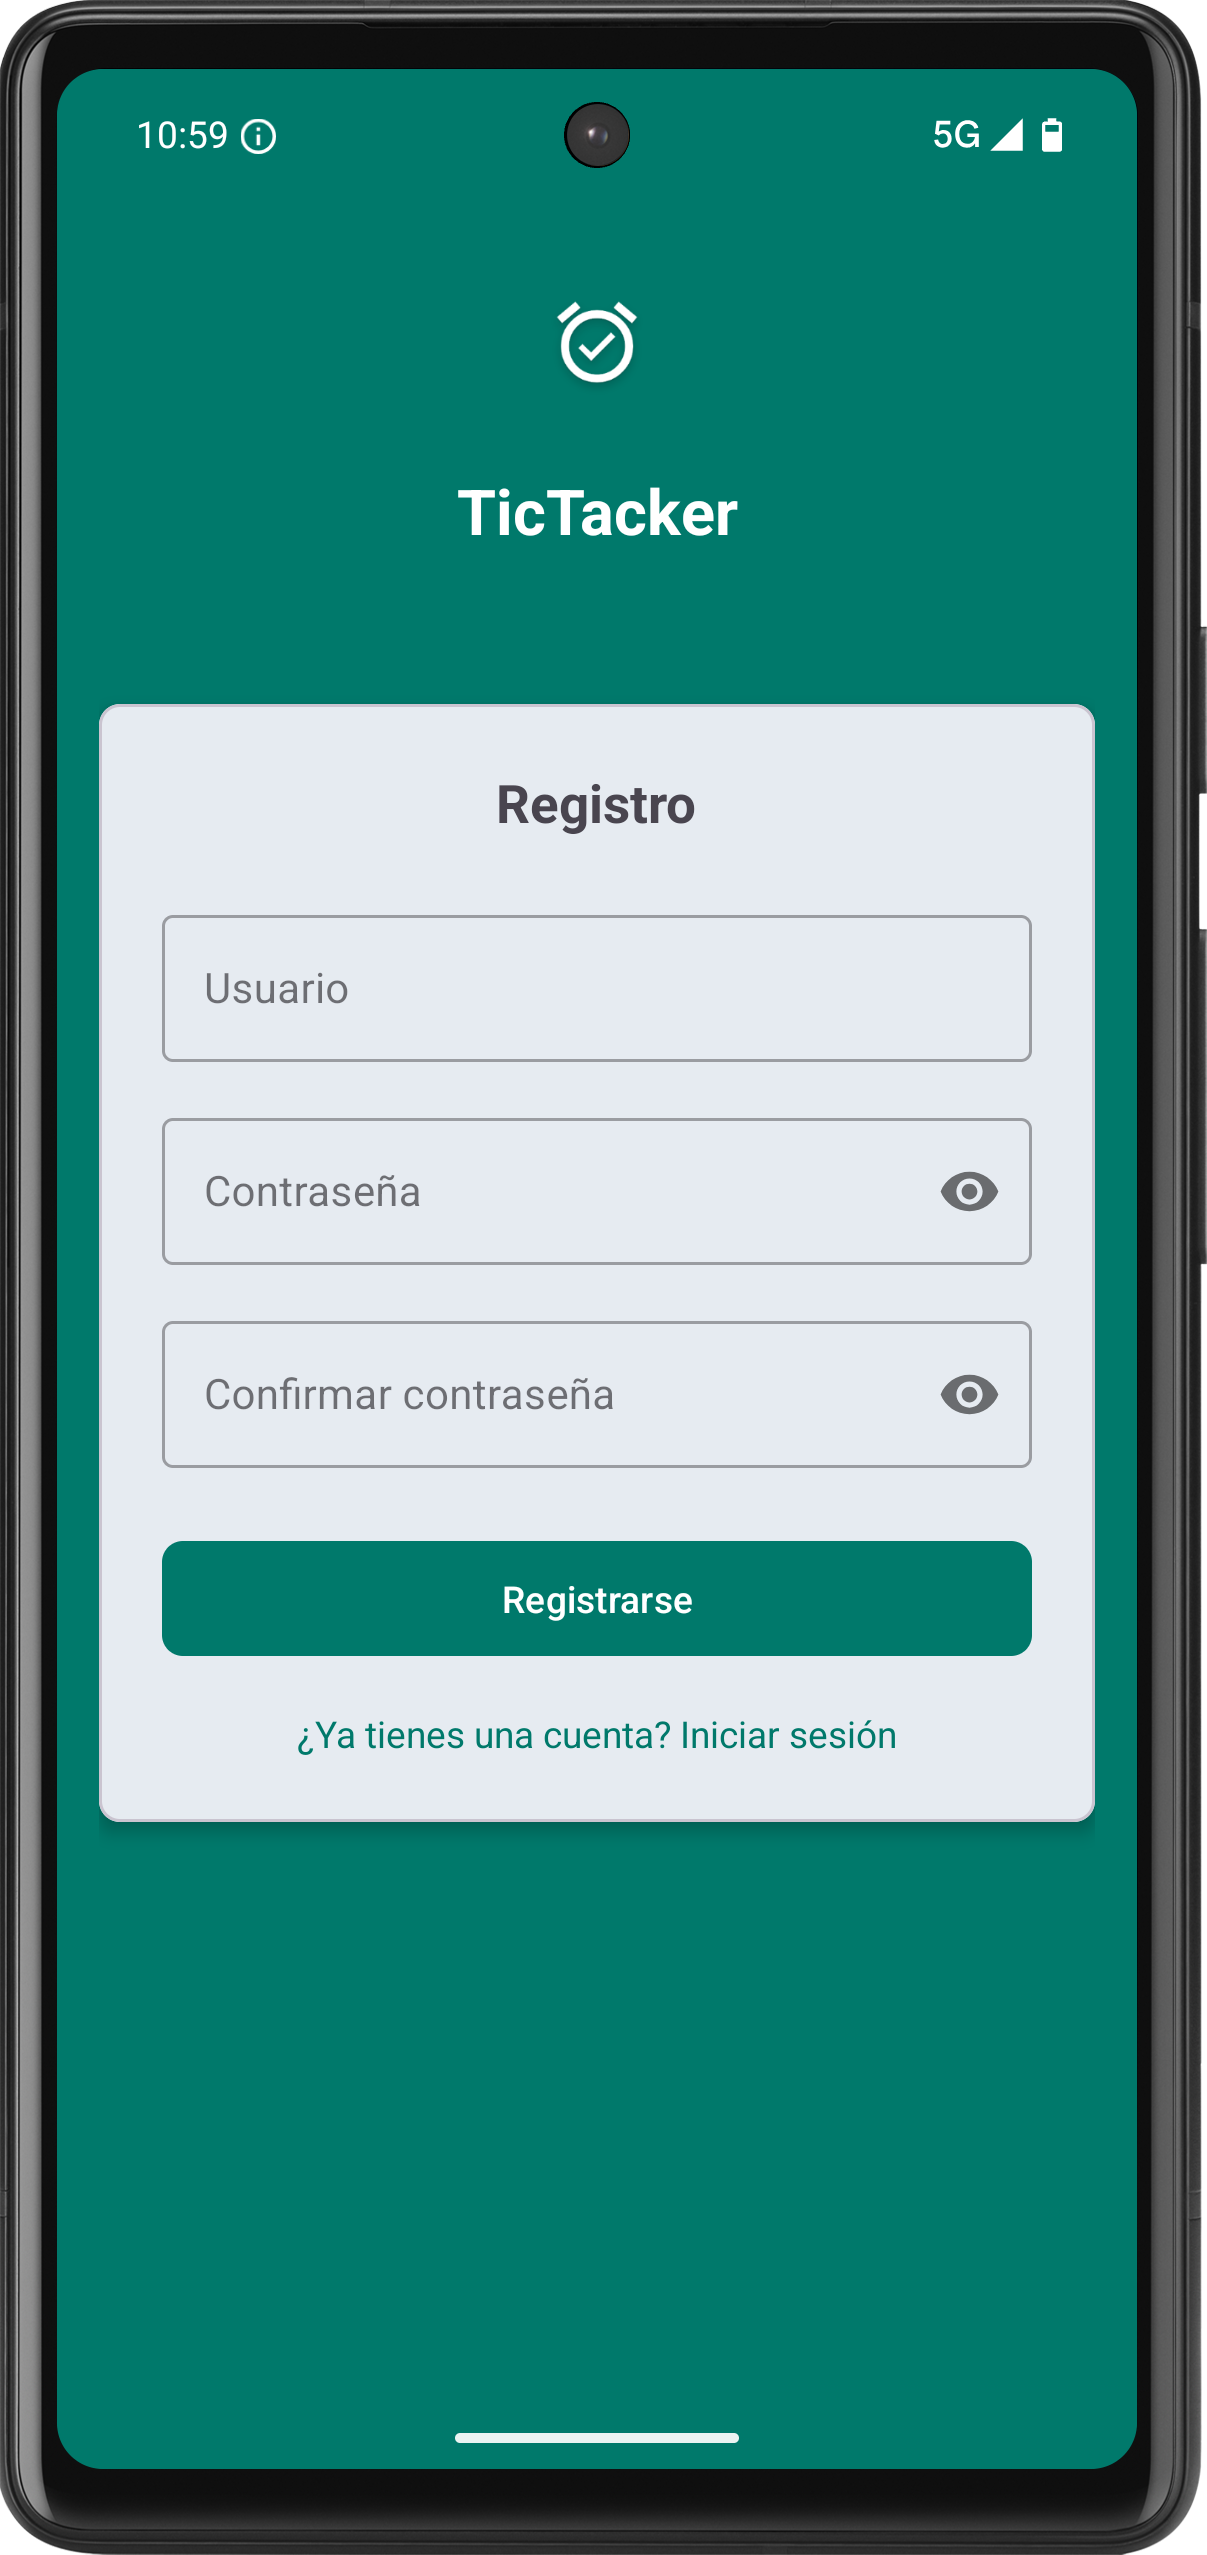
\includegraphics[width=\textwidth]{root/signup.png}
         \caption{Registro de usuario}
         \label{fig:signup}
     \end{subfigure}
     \hfill
     \begin{subfigure}[b]{0.3\textwidth}
         \centering
         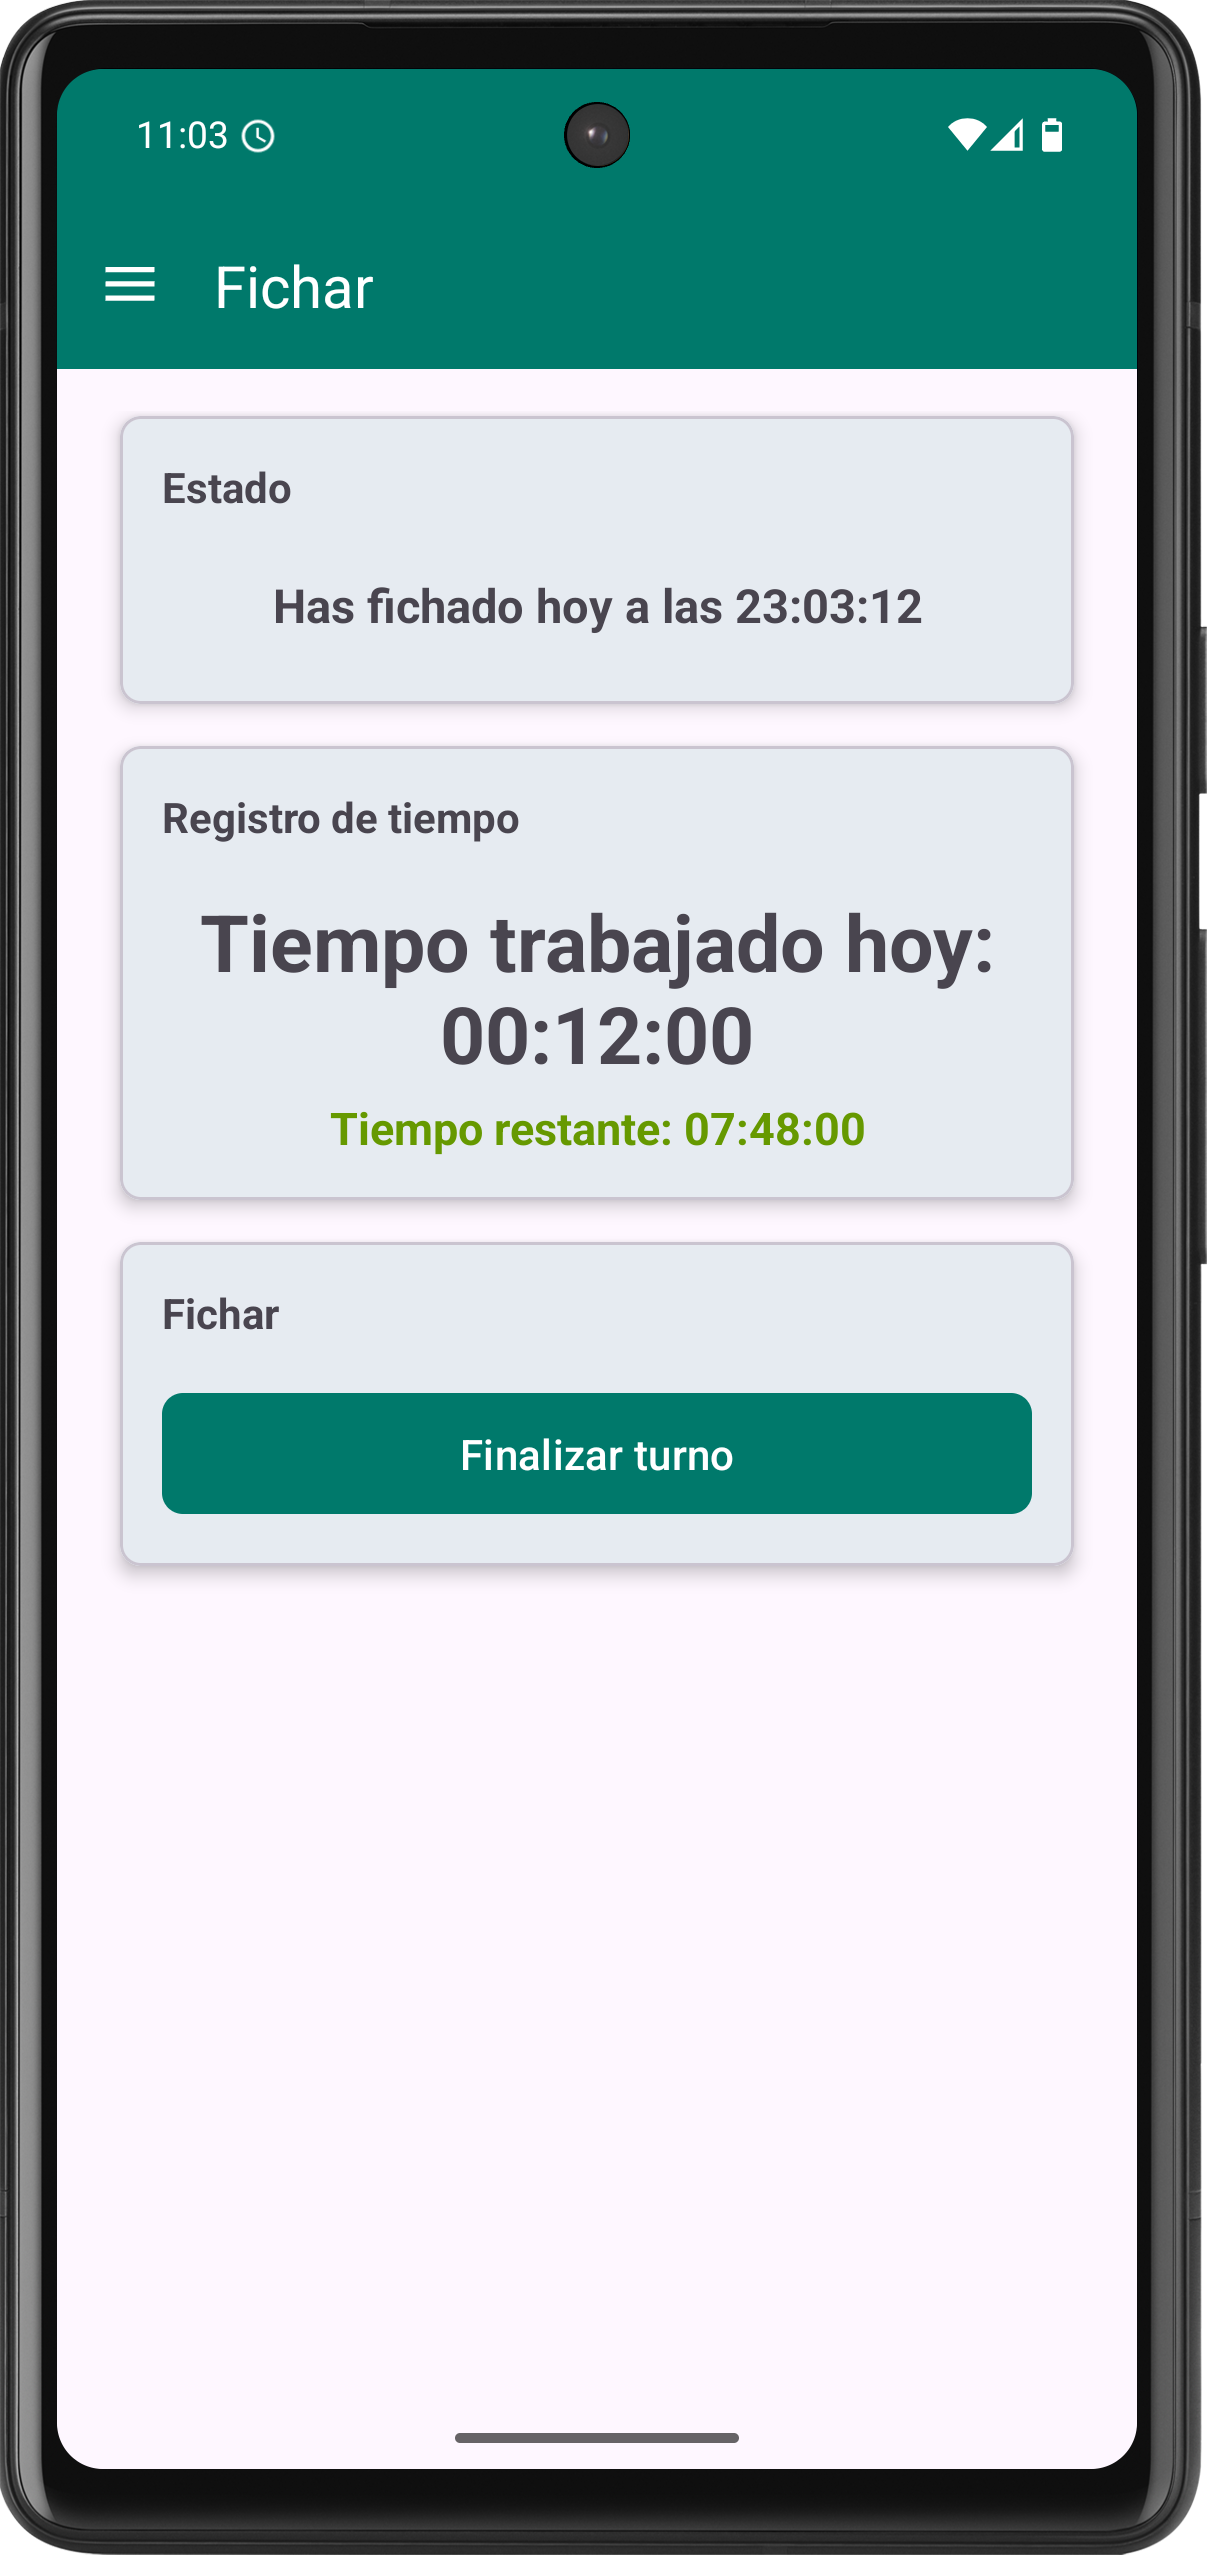
\includegraphics[width=\textwidth]{root/fichado.png}
         \caption{Pantalla de inicio}
         \label{fig:fichado}
     \end{subfigure}
        \caption{Pantalla de bienvenida e inicio de sesión}
        \label{fig:bienvenida}
\end{figure}

\subsection{Ajustes de la aplicación}

Pulsando sobre la sección de “Ajustes” en el menú de la aplicación, se accederá a la configuración. Es importante presionar sobre el botón de “Guardar” para que se refresque la vista de la aplicación y se puedan ver los cambios realizados de forma correcta si se modifica alguno de los campos.

Para obtener la mejor experiencia posible, se permite elegir, tal y como se muestra en la Figura \ref{fig:settings-1}, entre Español e Inglés como idiomas, siendo suficiente con elegir en el desplegable el preferido para configurarlo como el idioma por defecto para toda la aplicación. A continuación, el usuario deberá completar los datos de su jornada laboral, especificando los días laborables y las horas que se trabaja a la semana usando los controles. Esta información permite a la aplicación calcular las horas que se trabajará cada día, así como enviar notificaciones en caso de superar la previsión diaria y mostrar un cuadro de diálogo si se trata de salir antes de lo previsto. También se puede configurar una alerta para recordar fichar, de modo que si se alcanza dicha hora y no se ha registrado ningún fichaje, se recibirá una notificación. Esta funcionalidad hace uso de las alarmas programadas de Android, por lo que funciona incluso aunque la app esté cerrada, pero es preciso habilitar el permiso correspondiente.

De forma opcional, es posible incluir una imagen como logotipo, que se mostrará en el menú de la aplicación tal y como ilustra la Figura \ref{fig:settings-3}. Para ello, basta con pulsar sobre el botón de “Cambiar” y elegir el nuevo logotipo en el explorador, como muestra la Figura \ref{fig:settings-2}. Debe ser un fichero de imagen, y se recomienda que sea un PNG con fondo transparente y un color claro para mejor visibilidad. En caso de querer restaurar el logotipo por defecto, puede usarse el botón de “Quitar”.

De forma adicional, esta pantalla también permite cerrar sesión para cambiar de usuario, lo que nos llevaría directamente a la pantalla de inicio de sesión, así como eliminar los datos de fichaje almacenados, lo que no se recomienda salvo que se hayan exportado previamente.

\begin{figure}[H]
     \centering
     \begin{subfigure}[b]{0.3\textwidth}
         \centering
         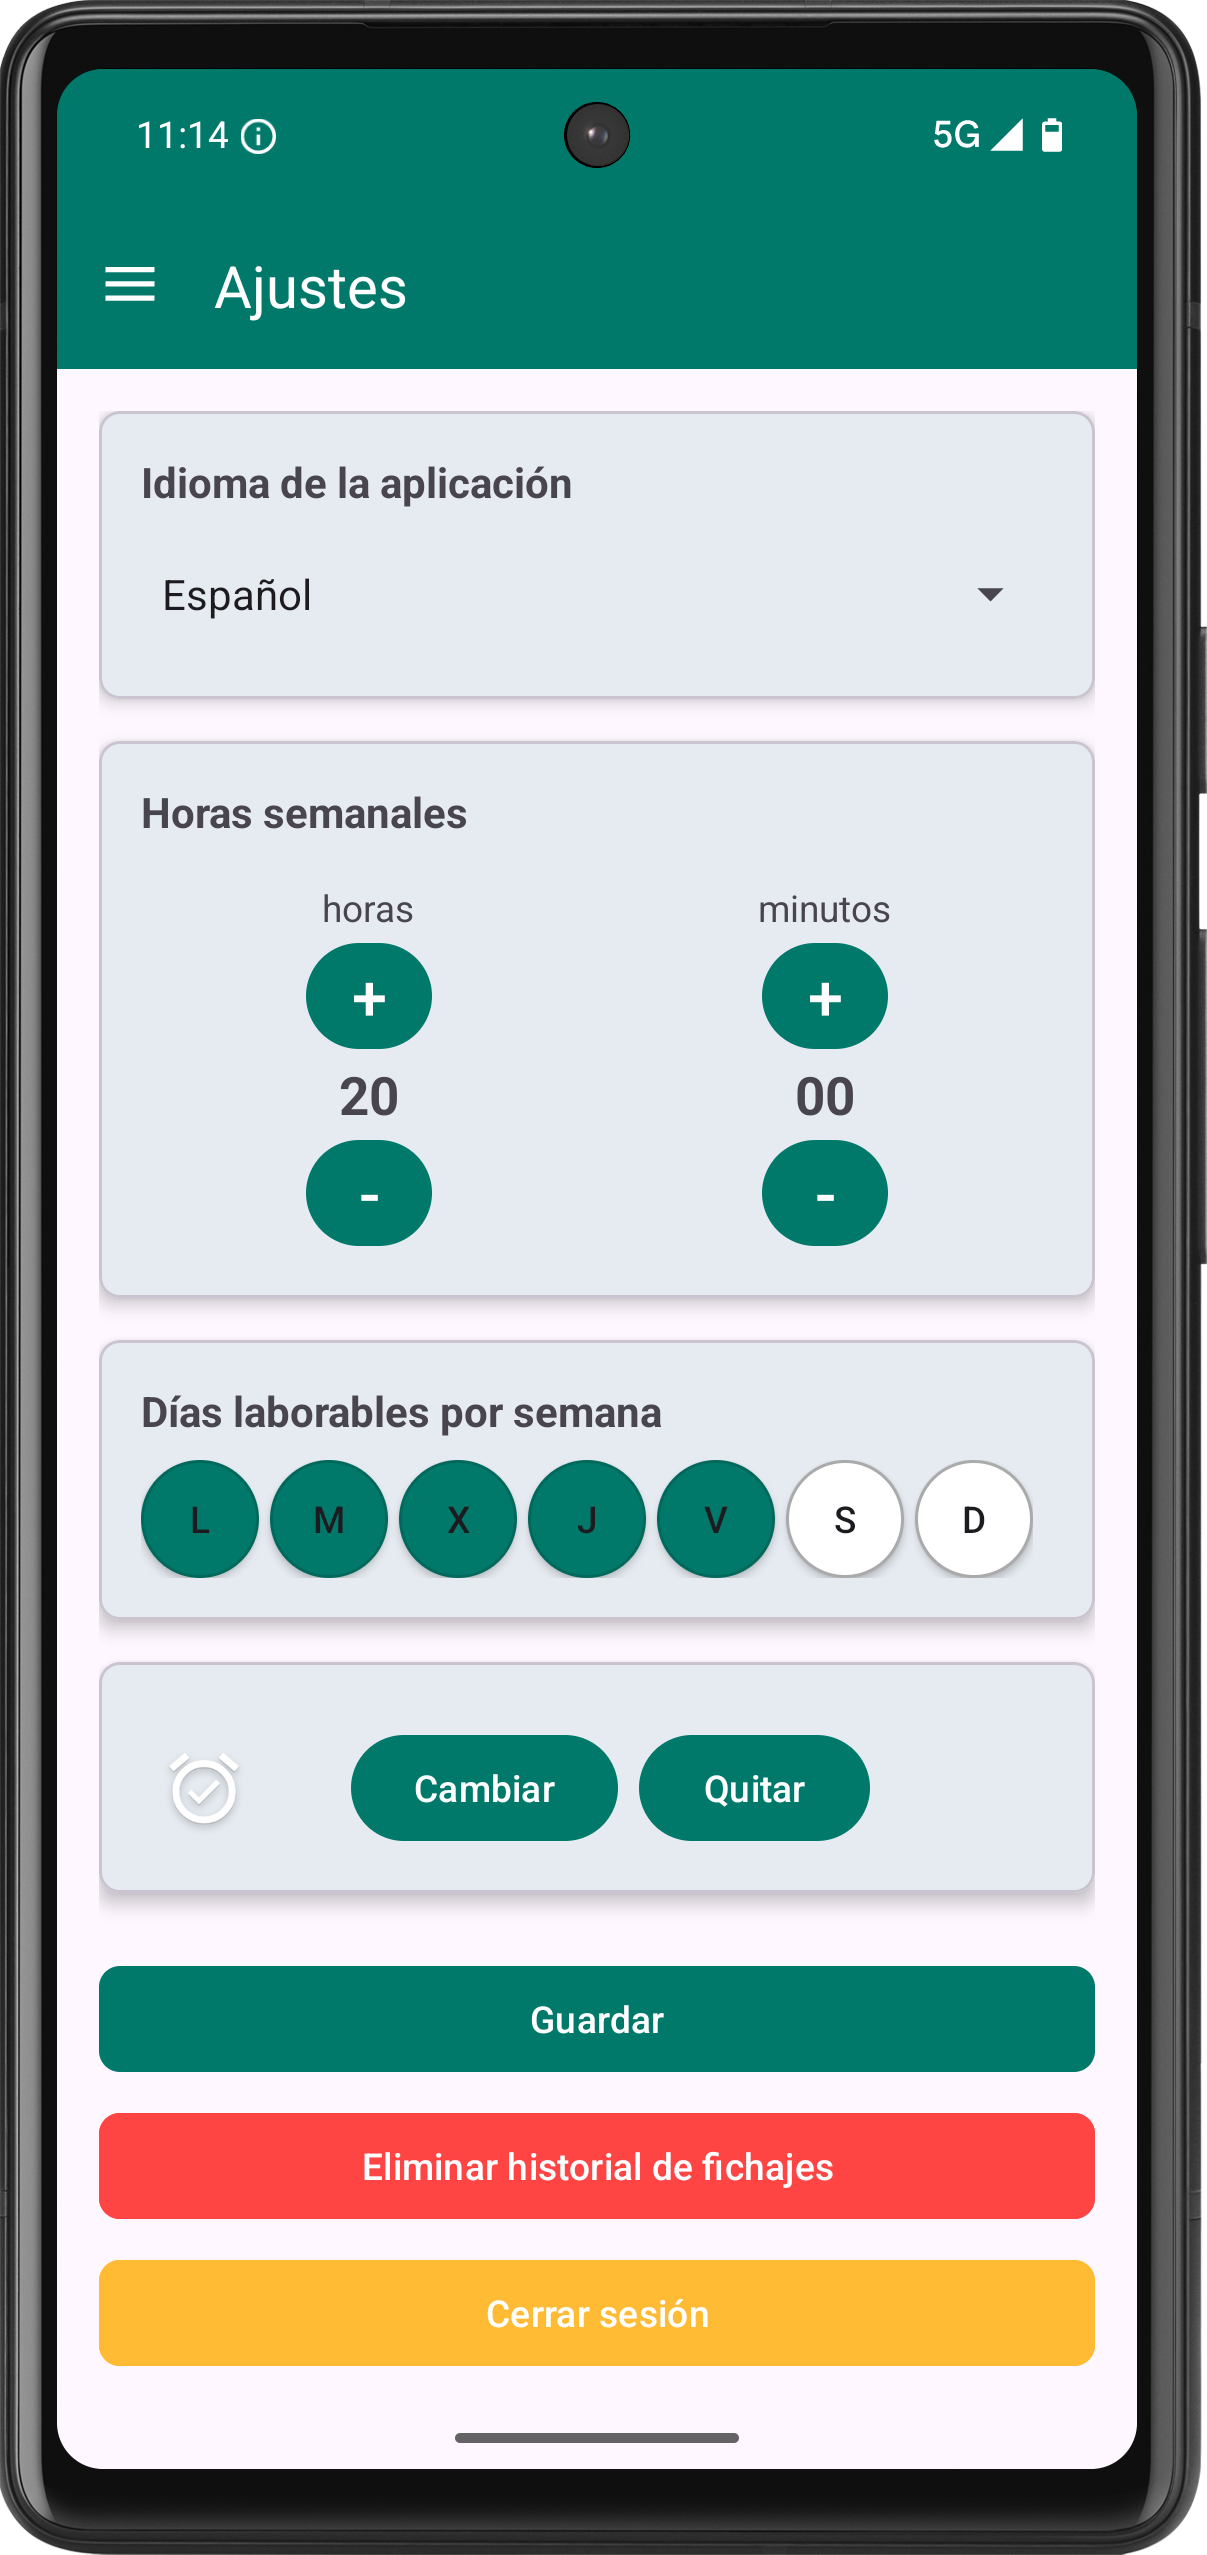
\includegraphics[width=\textwidth]{root/settings-1.png}
         \caption{Ajustes de la aplicación}
         \label{fig:settings-1}
     \end{subfigure}
     \hfill
     \begin{subfigure}[b]{0.3\textwidth}
         \centering
         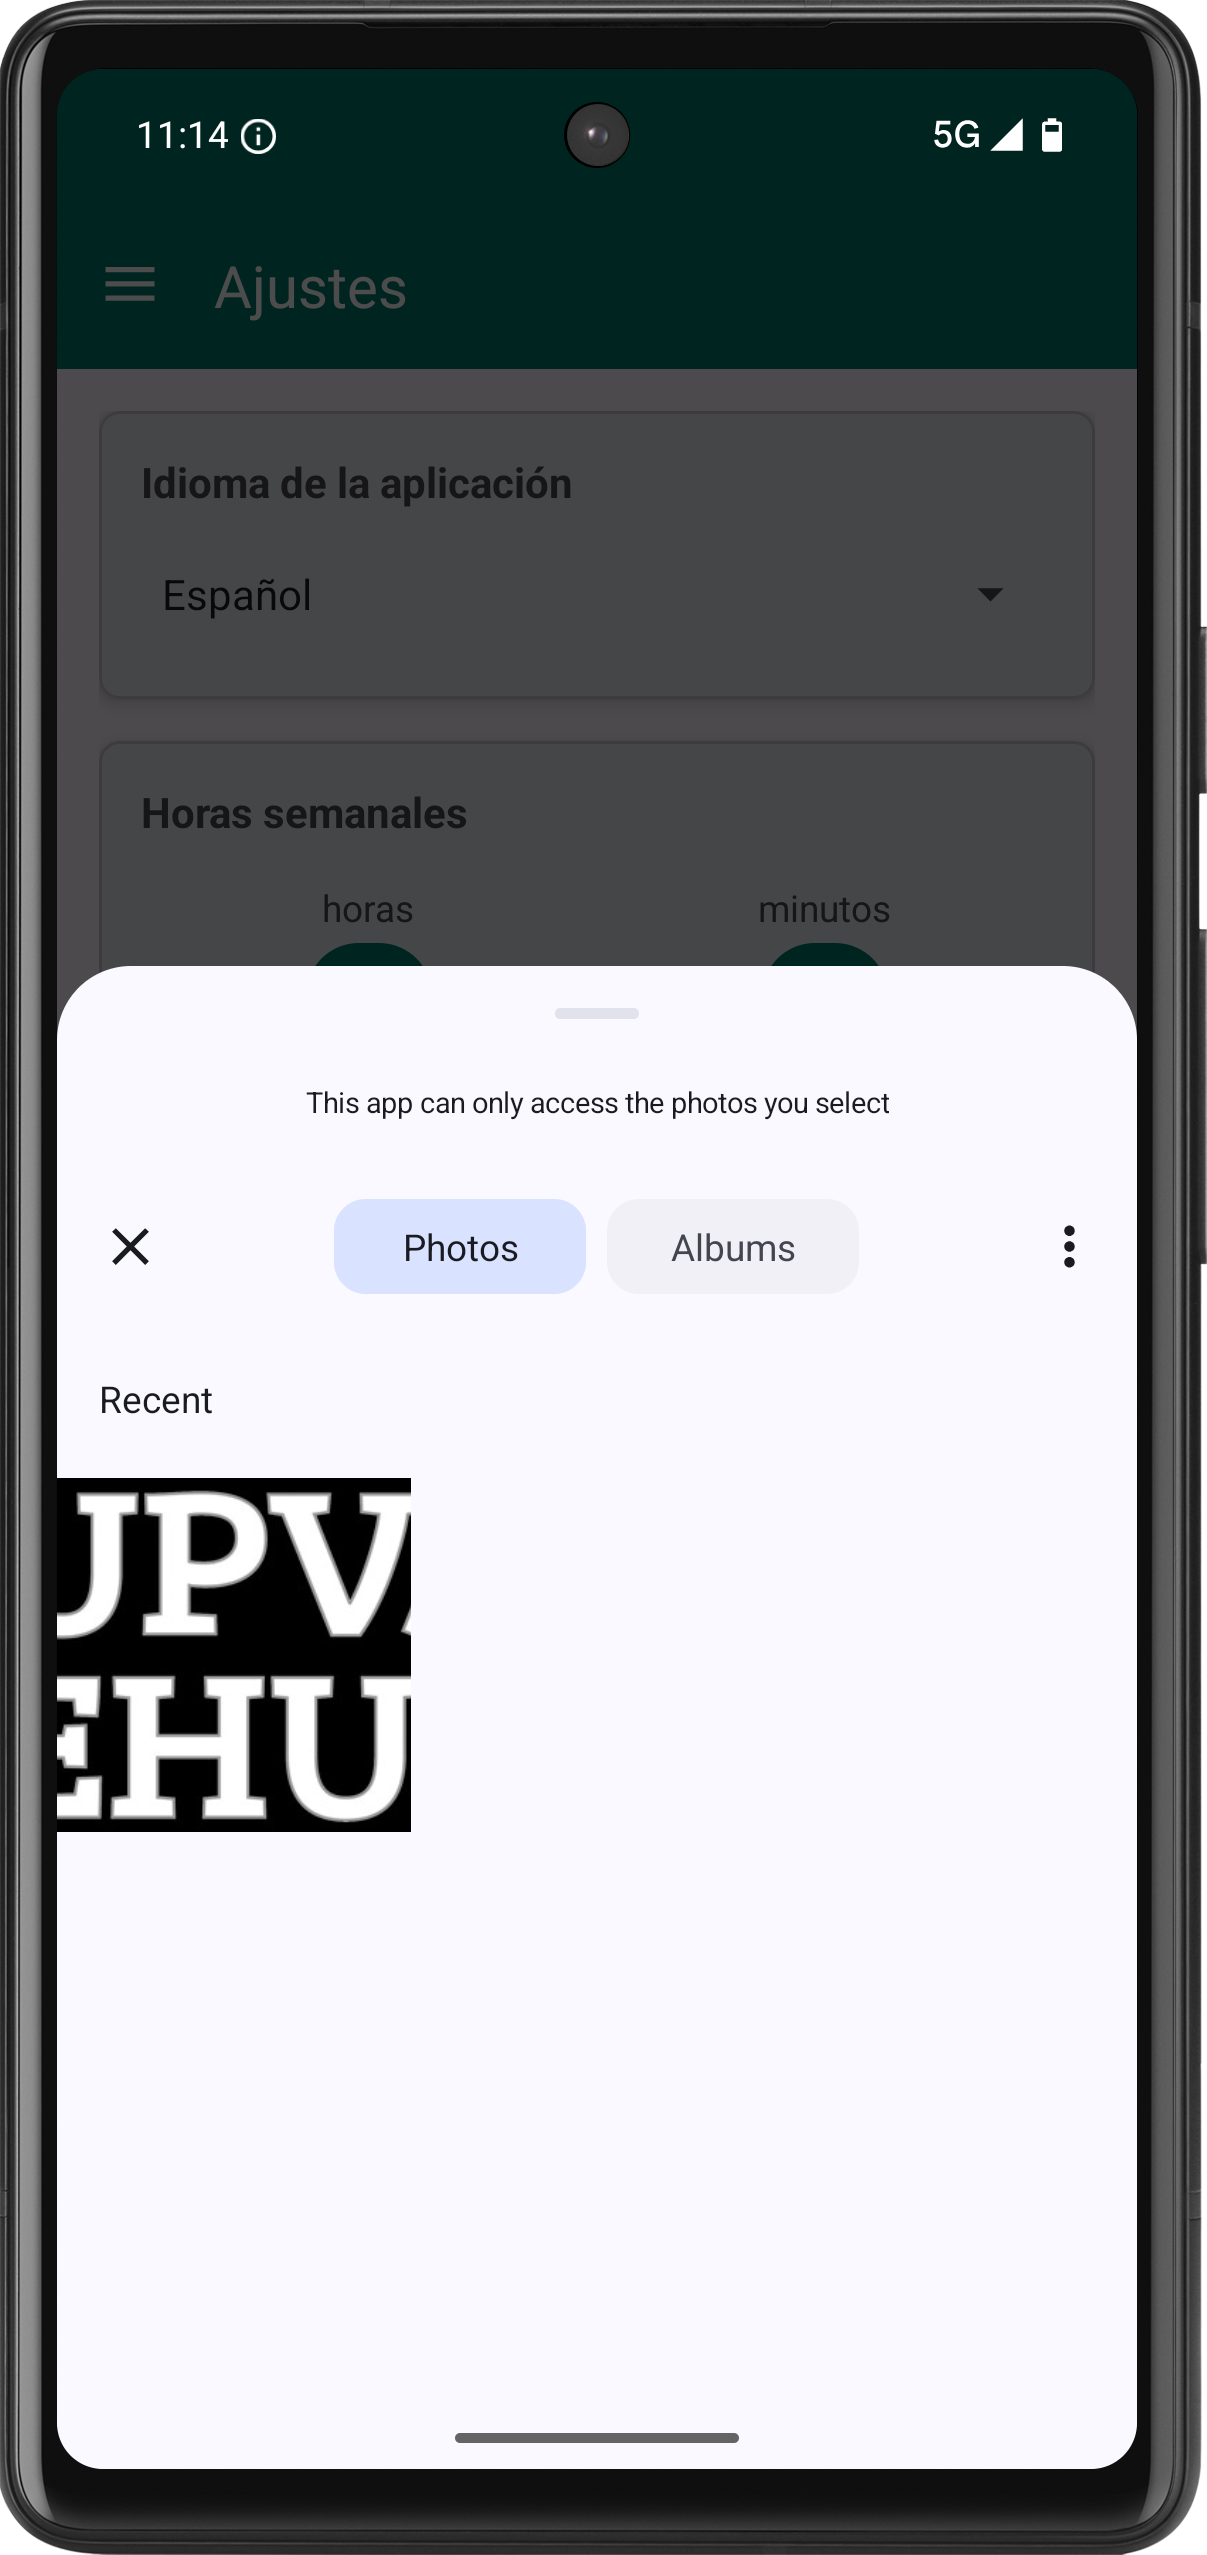
\includegraphics[width=\textwidth]{root/settings-2.png}
         \caption{Selección de nuevo logotipo}
         \label{fig:settings-2}
     \end{subfigure}
     \hfill
     \begin{subfigure}[b]{0.3\textwidth}
         \centering
         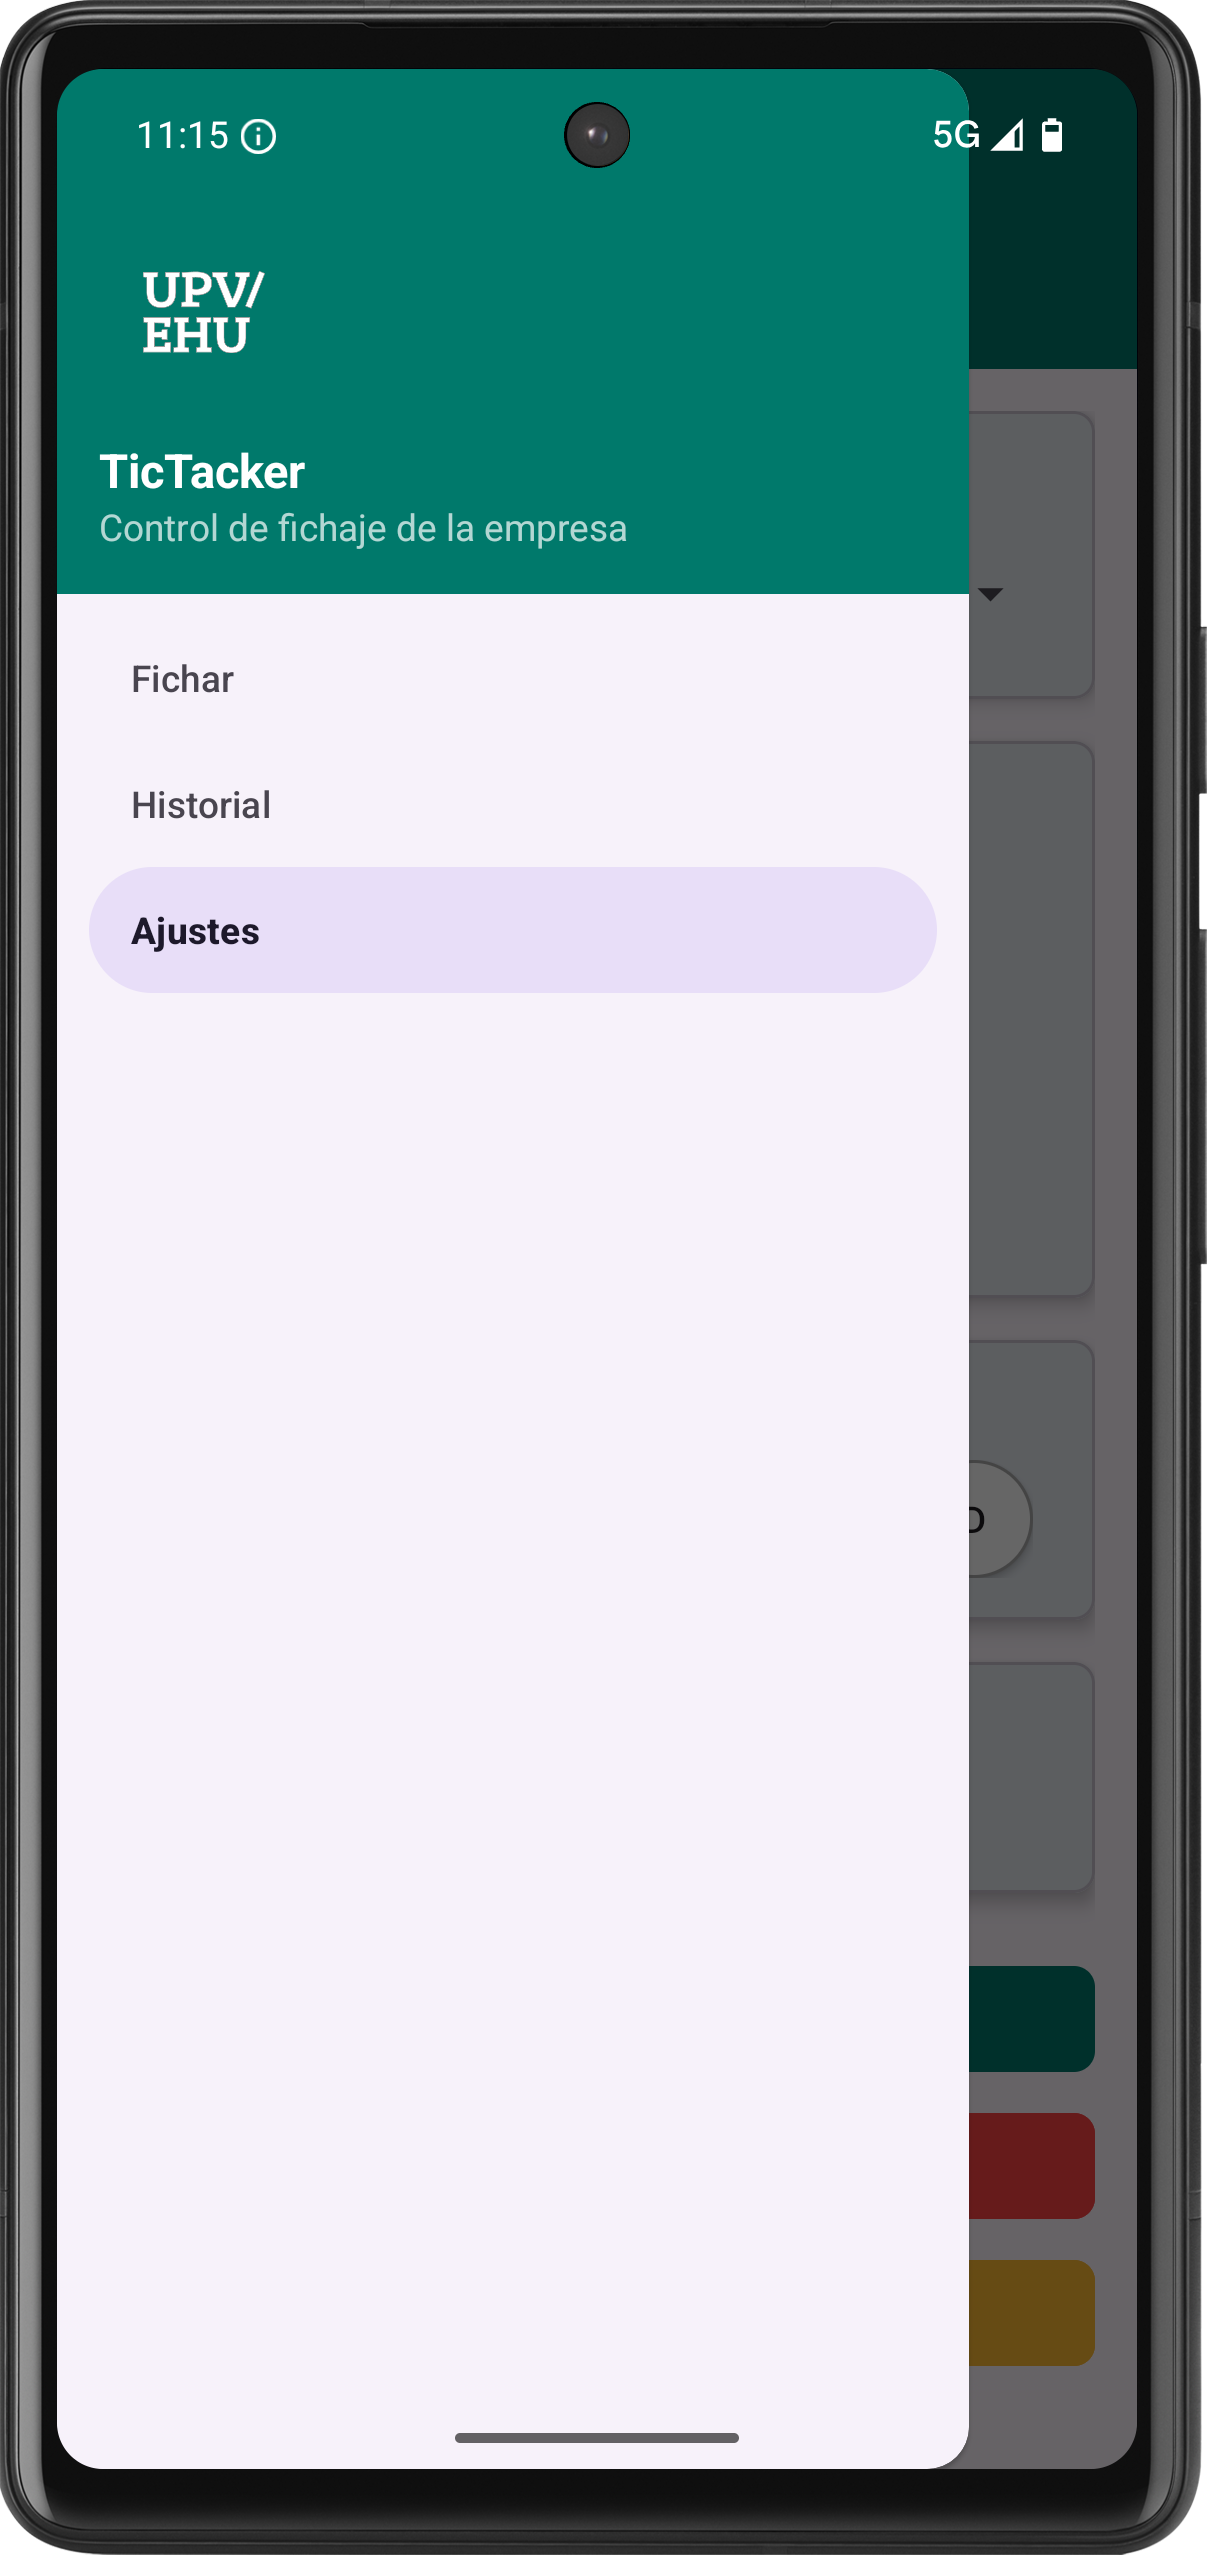
\includegraphics[width=\textwidth]{root/settings-3.png}
         \caption{Navegación con logotipo}
         \label{fig:settings-3}
     \end{subfigure}
        \caption{Ajustes de la aplicación}
        \label{fig:bienvenida}
\end{figure}

\subsection{Fichajes e historial}

Accediendo a la pantalla para fichar, es posible consultar de un vistazo los datos de un fichaje activo, tal y como muestra la Figura \ref{fig:fichando}. Es posible marcar una entrada y una salida por medio del botón asociado de forma sencilla, y consultar la hora, minuto y segundo exacto en el que se fichó, así como la duración actual, el tiempo restante para alcanzar la jornada o, en su defecto, las horas extraordinarias realizadas. Al llegar a las horas estimadas, se recibe una notificación si la aplicación está activa.

Además, durante el tiempo de fichaje, como se gestiona en primer plano, se muestra una notificación persistente silenciosa que permite conocer en tiempo real el tiempo durante el que se ha fichado. Además, tal y como se muestra en la Figura \ref{fig:widget}, se ha incluido también un widget que se actualiza de forma dinámica y que permite fichar o salir con un solo clic, o bien consultar el tiempo fichado y restante. Añadir el widget a la pantalla de inicio varía según el dispositivo usado.

Una vez guardado el fichaje, desde el menú es posible acceder al historial que muestra la figura \ref{fig:historial}. En él, puede verse un registro de todos los fichajes almacenados en la aplicación, mostrándose primero el más reciente. Si se pulsa sobre uno de ellos, como se muestra en la Figura \ref{fig:detalles}, es posible ver el detalle completo, consultando la fecha y hora exactas de salidas y entradas, así como las coordenadas geográficas desde las que se produjo el fichaje en caso de haber otorgado permisos para acceder a la ubicación (en su defecto, se mostrará que no está disponible), y un mapa de OpenStreetMap que permite ver dicha ubicación.

En la parte inferior de la ventana de detalles, existen opciones para editar un fichaje guardado, que permite modificar la hora de entrada o salida en caso de haberse identificado algún error, así como la opción de ver en un mapa la ubicación registrada. Al pulsar sobre esta opción, se abre la aplicación de mapas asociada del dispositivo (Google Maps en gran parte de las ocasiones).

Indicar también que, al finalizar un fichaje, se añade también un evento al calendario para reflejarlo, en el que se detalla el usuario y el tiempo de la jornada. En la mayoría de casos, se añadirá al calendario predeterminado pero, en caso de no haber ninguno disponible con permisos de escritura, se creará un nuevo calendario con el nombre “TicTacker”. Como en las últimas versiones de Android este \textit{content provider} va ligado con las cuentas, es posible que el teléfono solicite acceso a los Contactos para realizar la tarea.

De forma adicional, la parte inferior de la aplicación permite importar o exportar una hoja de fichajes. Al presionar sobre exportar, se genera un fichero CSV con los fichados registrados, para el que deberá elegirse una ubicación dentro del dispositivo en la que guardarlo, mientras que si se selecciona importar, se puede elegir un fichero generado previamente por la aplicación o de forma manual con el mismo formato. Al hacerlo, se almacenarán los detalles en la base de datos y se podrá ver en el historial junto al resto de datos.

\begin{figure}[H]
     \centering
     \begin{subfigure}[b]{0.22\textwidth}
         \centering
         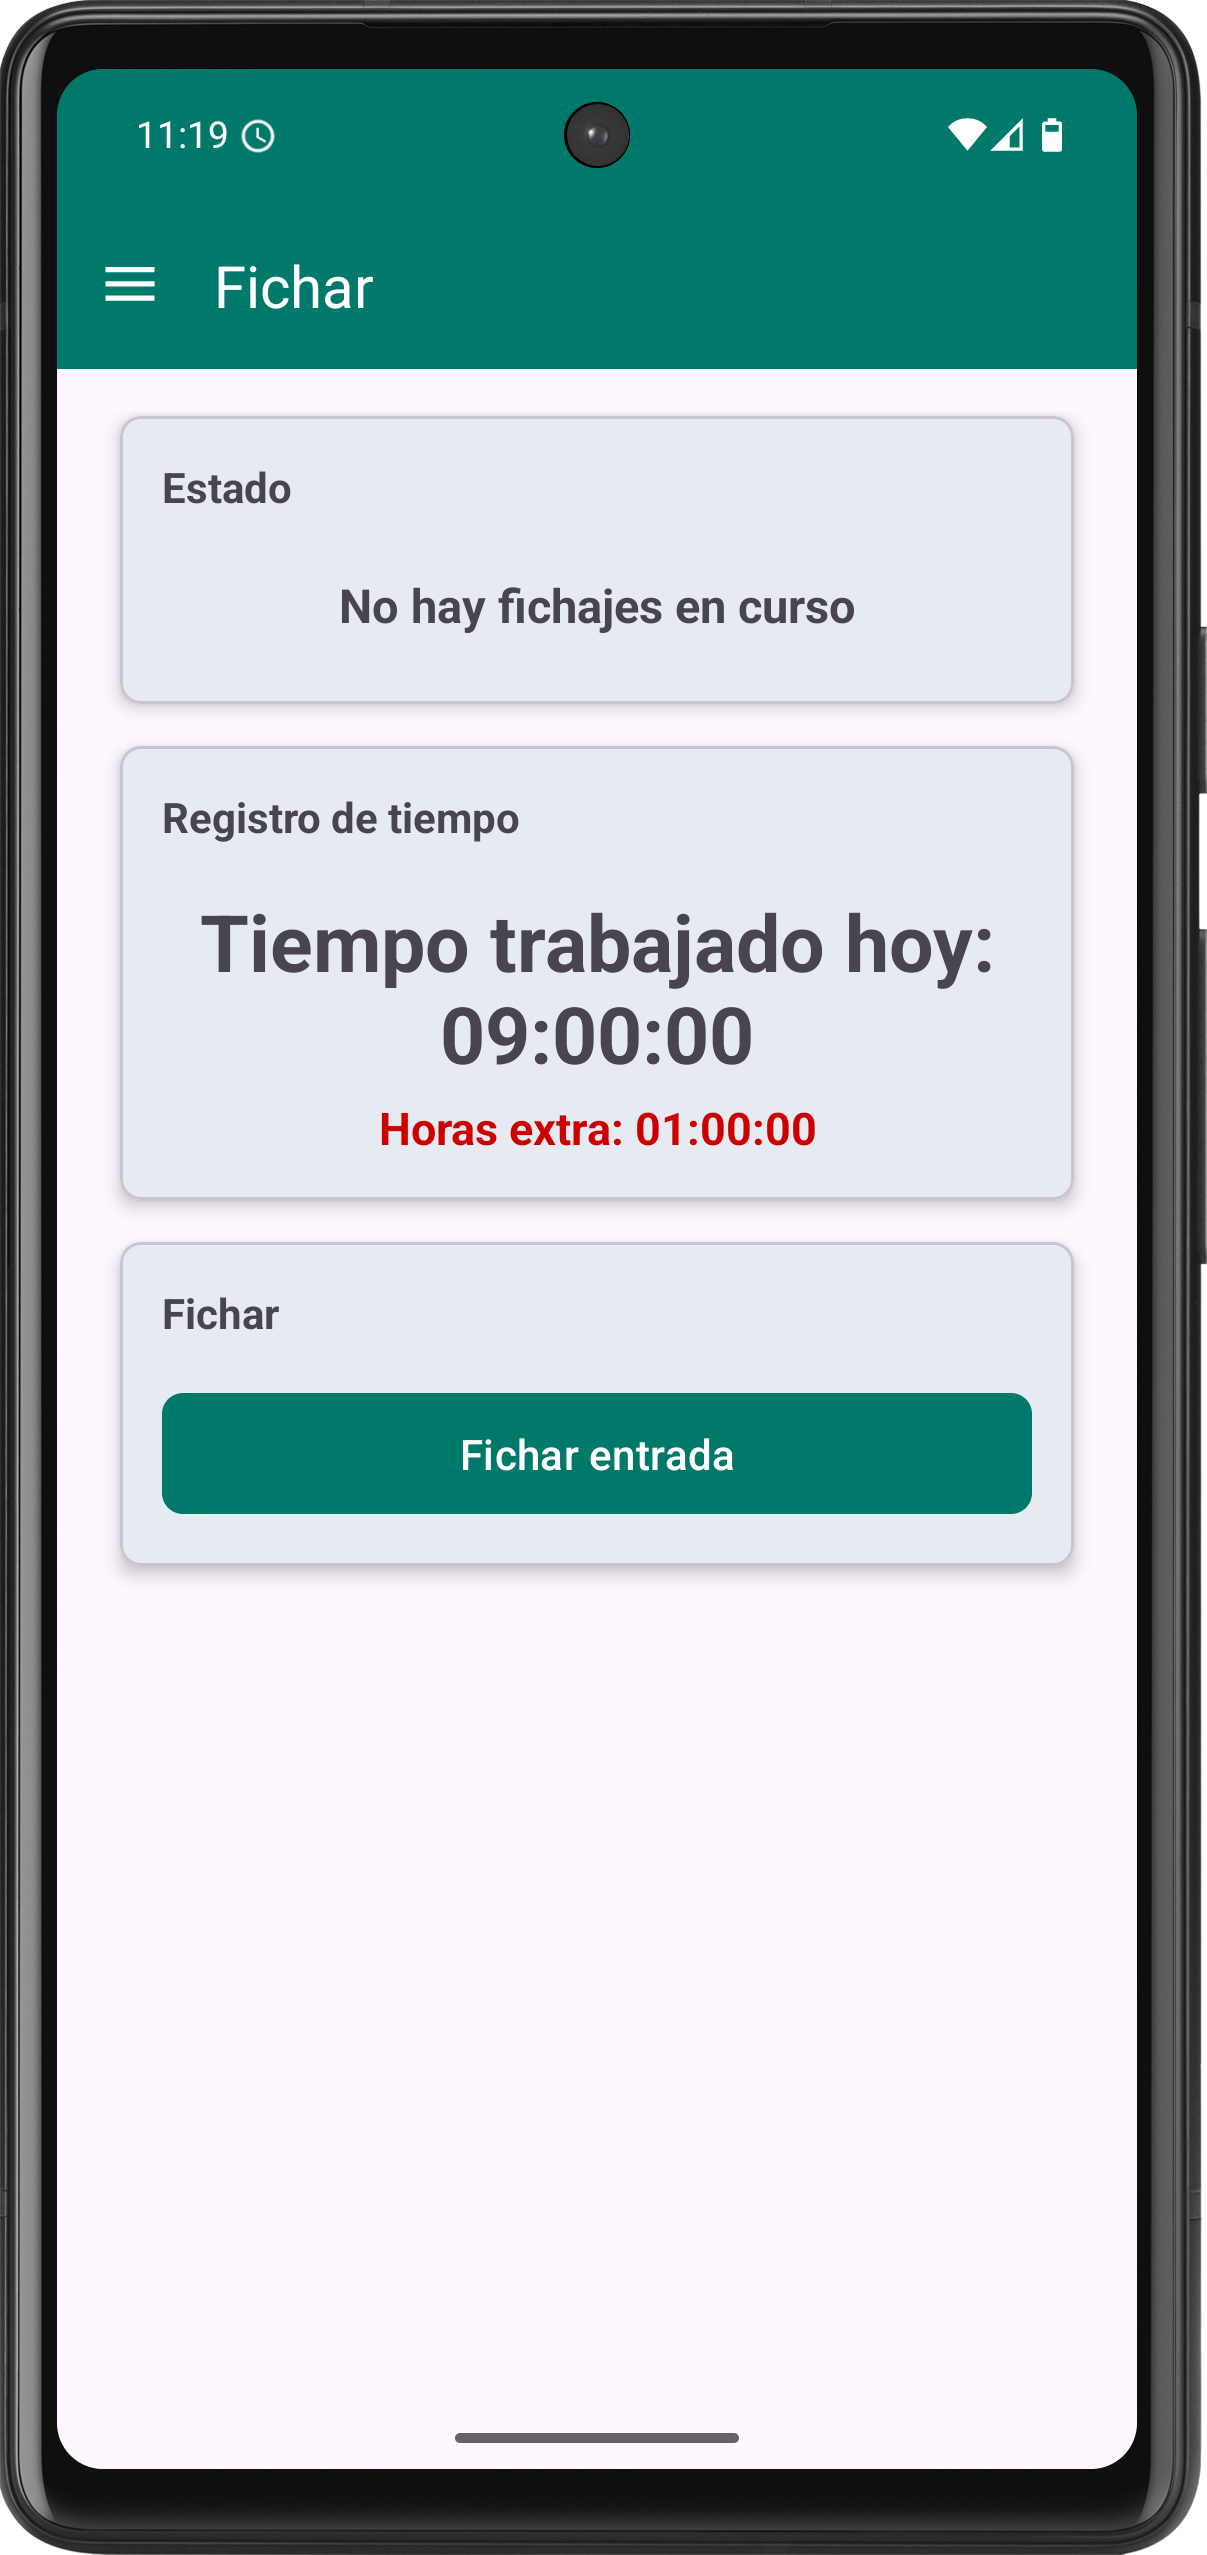
\includegraphics[width=\textwidth]{root/fichando.png}
         \caption{Pantalla principal}
         \label{fig:fichando}
     \end{subfigure}
     \hfill
     \begin{subfigure}[b]{0.22\textwidth}
         \centering
         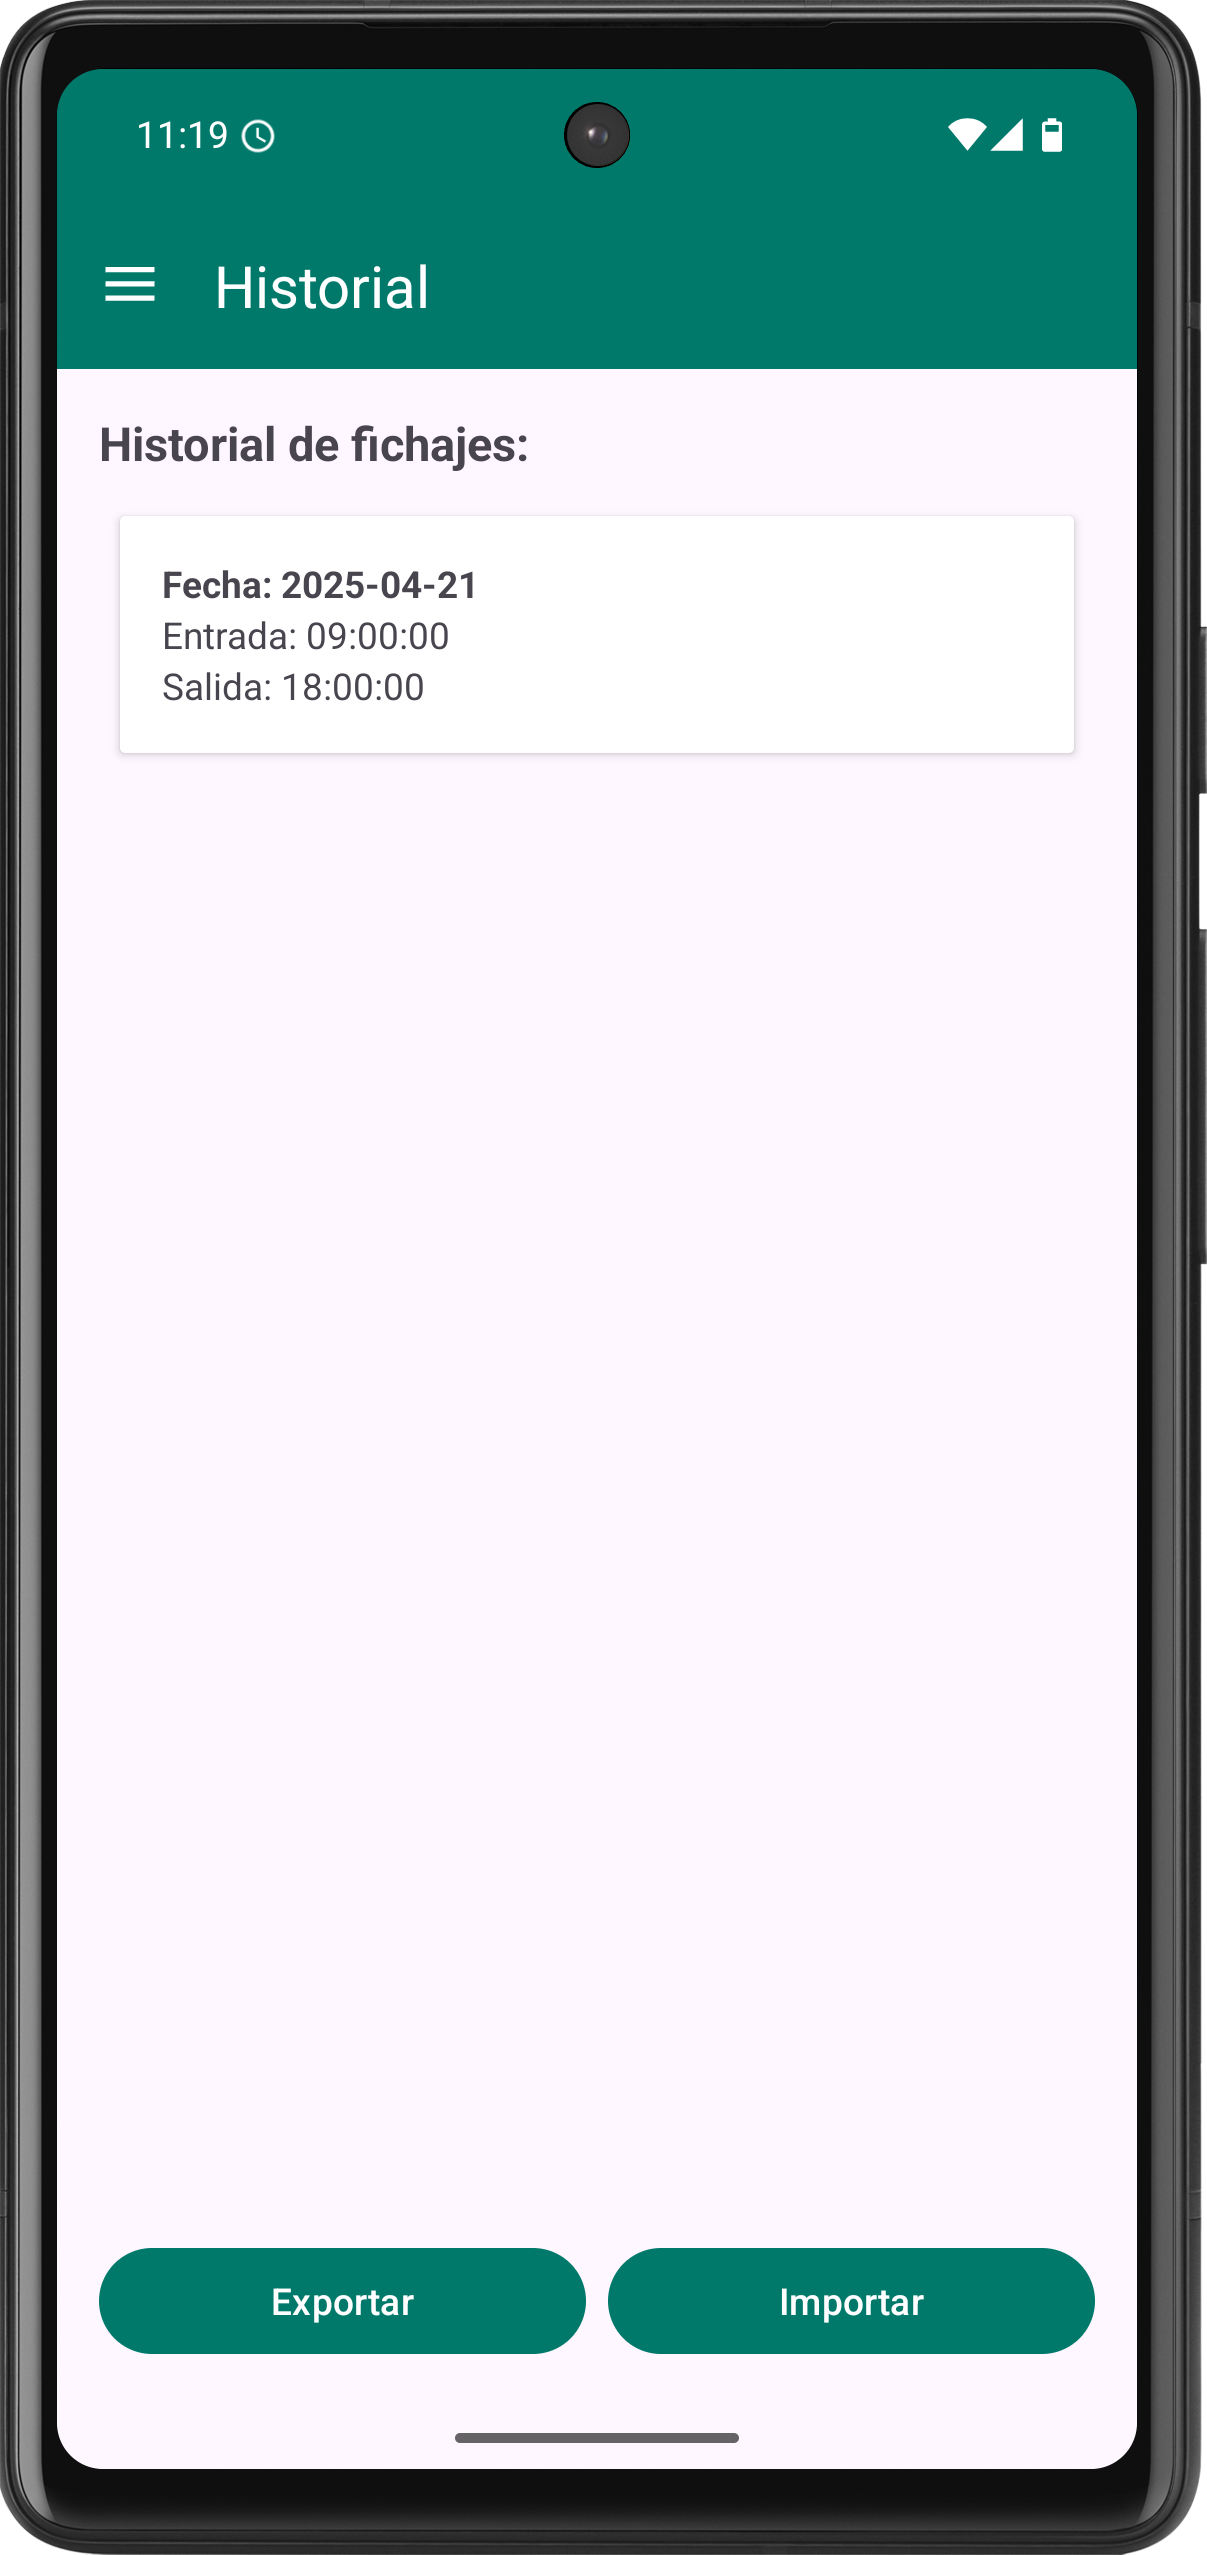
\includegraphics[width=\textwidth]{root/historial.png}
         \caption{Historial de fichajes}
         \label{fig:historial}
     \end{subfigure}
     \hfill
     \begin{subfigure}[b]{0.22\textwidth}
         \centering
         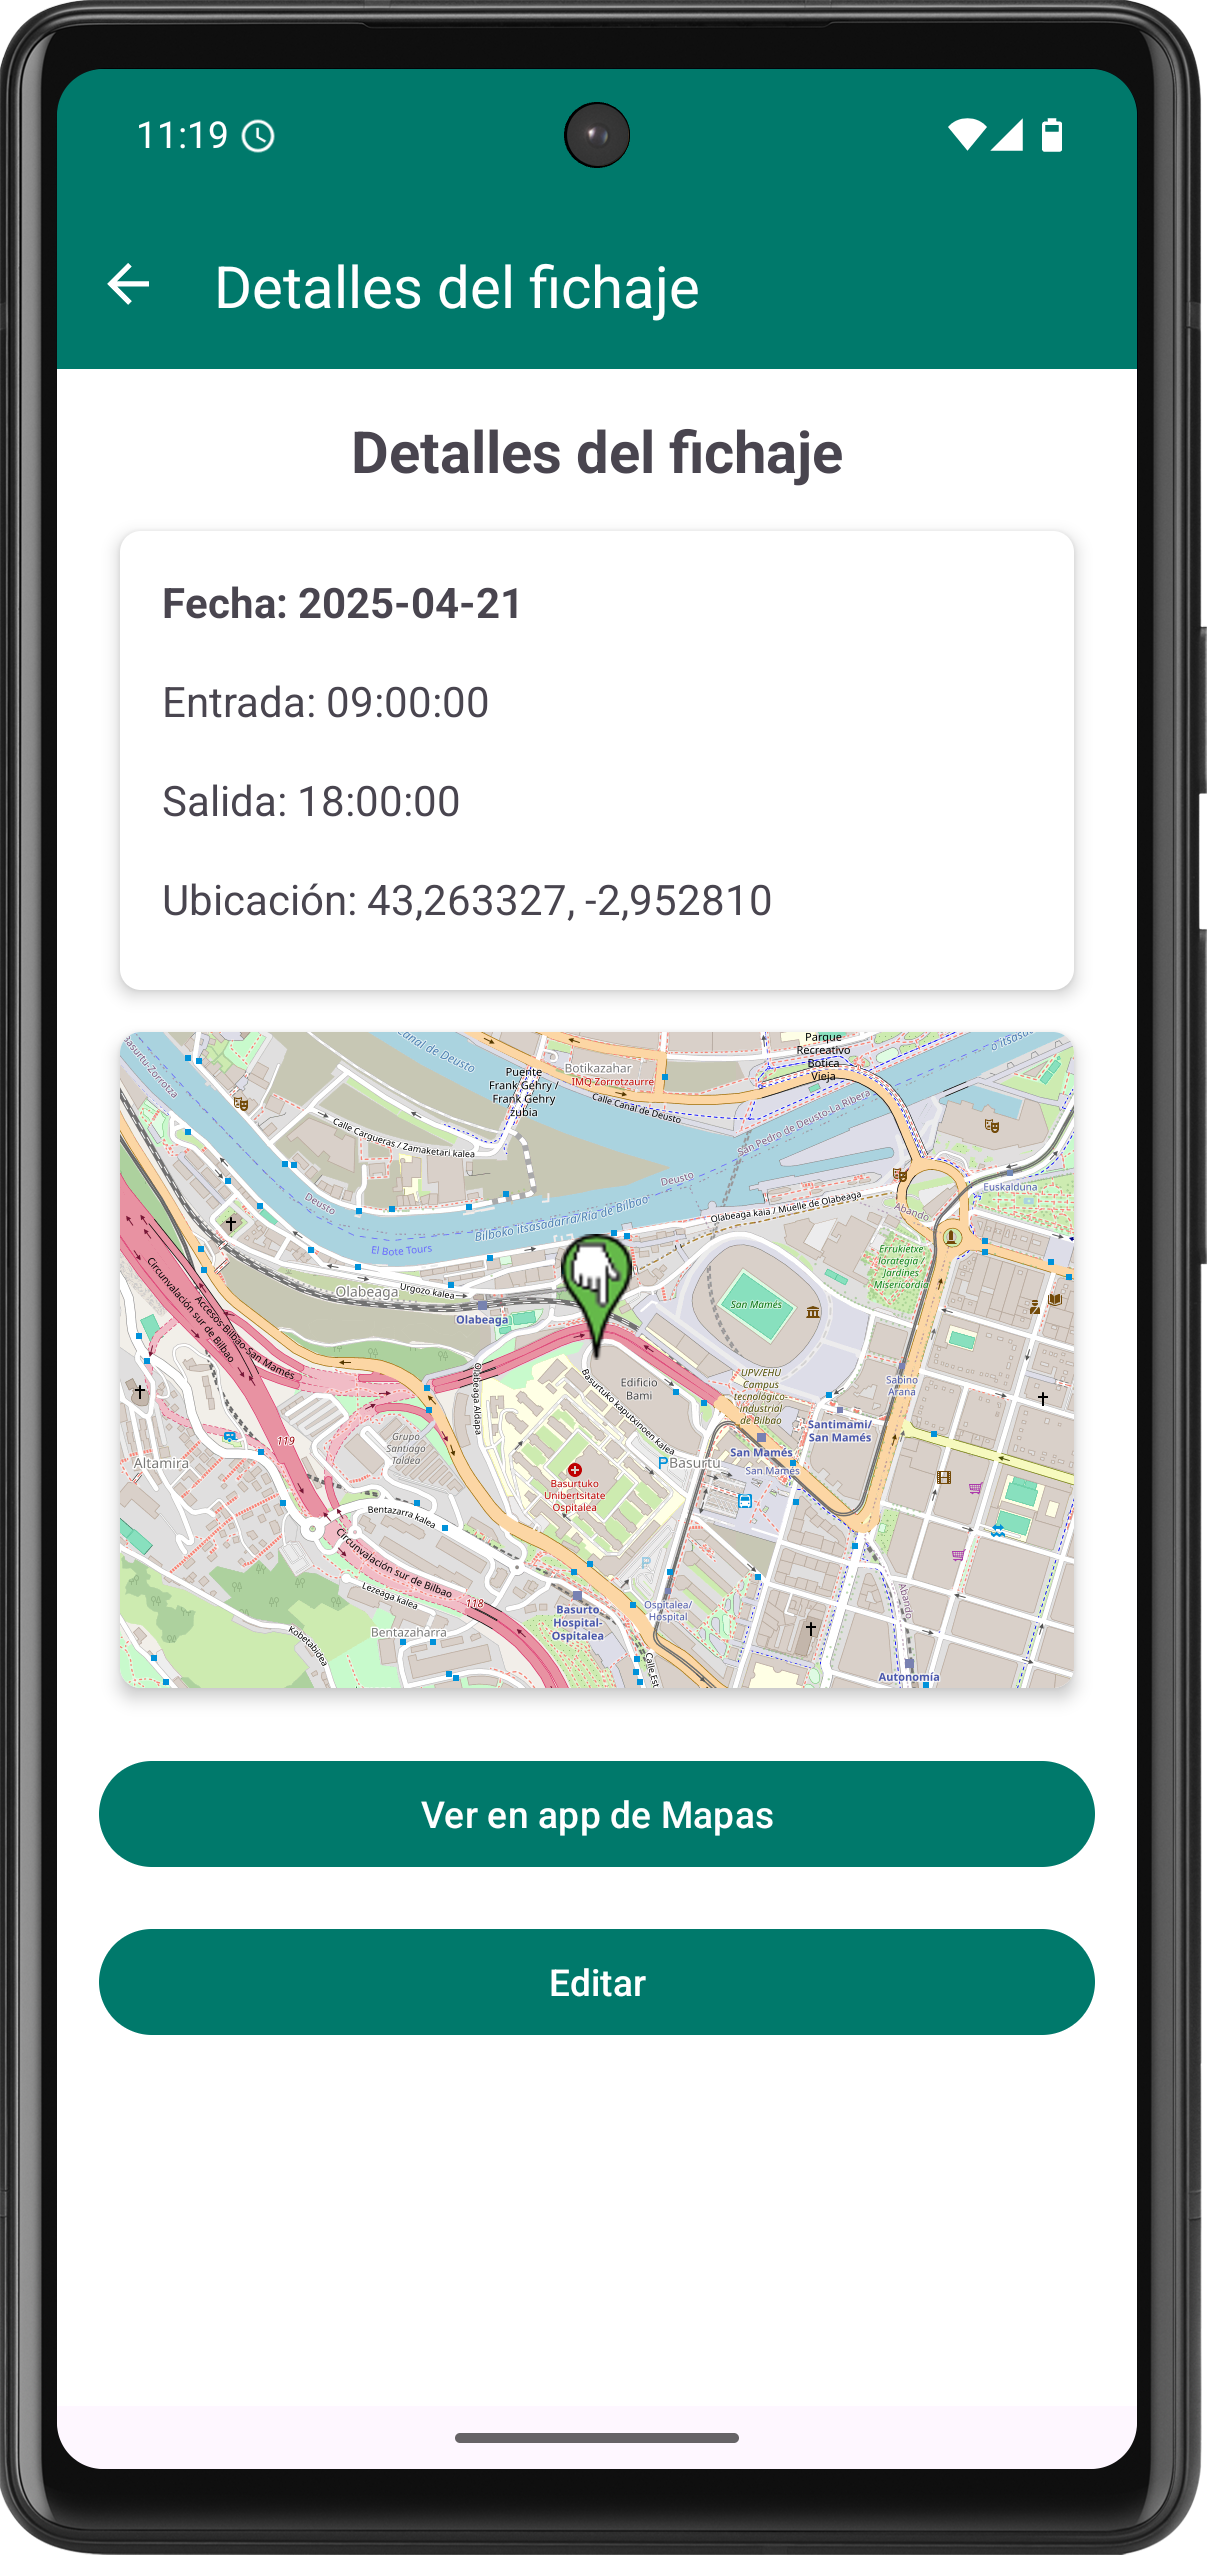
\includegraphics[width=\textwidth]{root/detalles.png}
         \caption{Detalles de un fichaje}
         \label{fig:detalles}
     \end{subfigure}
     \hfill
     \begin{subfigure}[b]{0.22\textwidth}
         \centering
         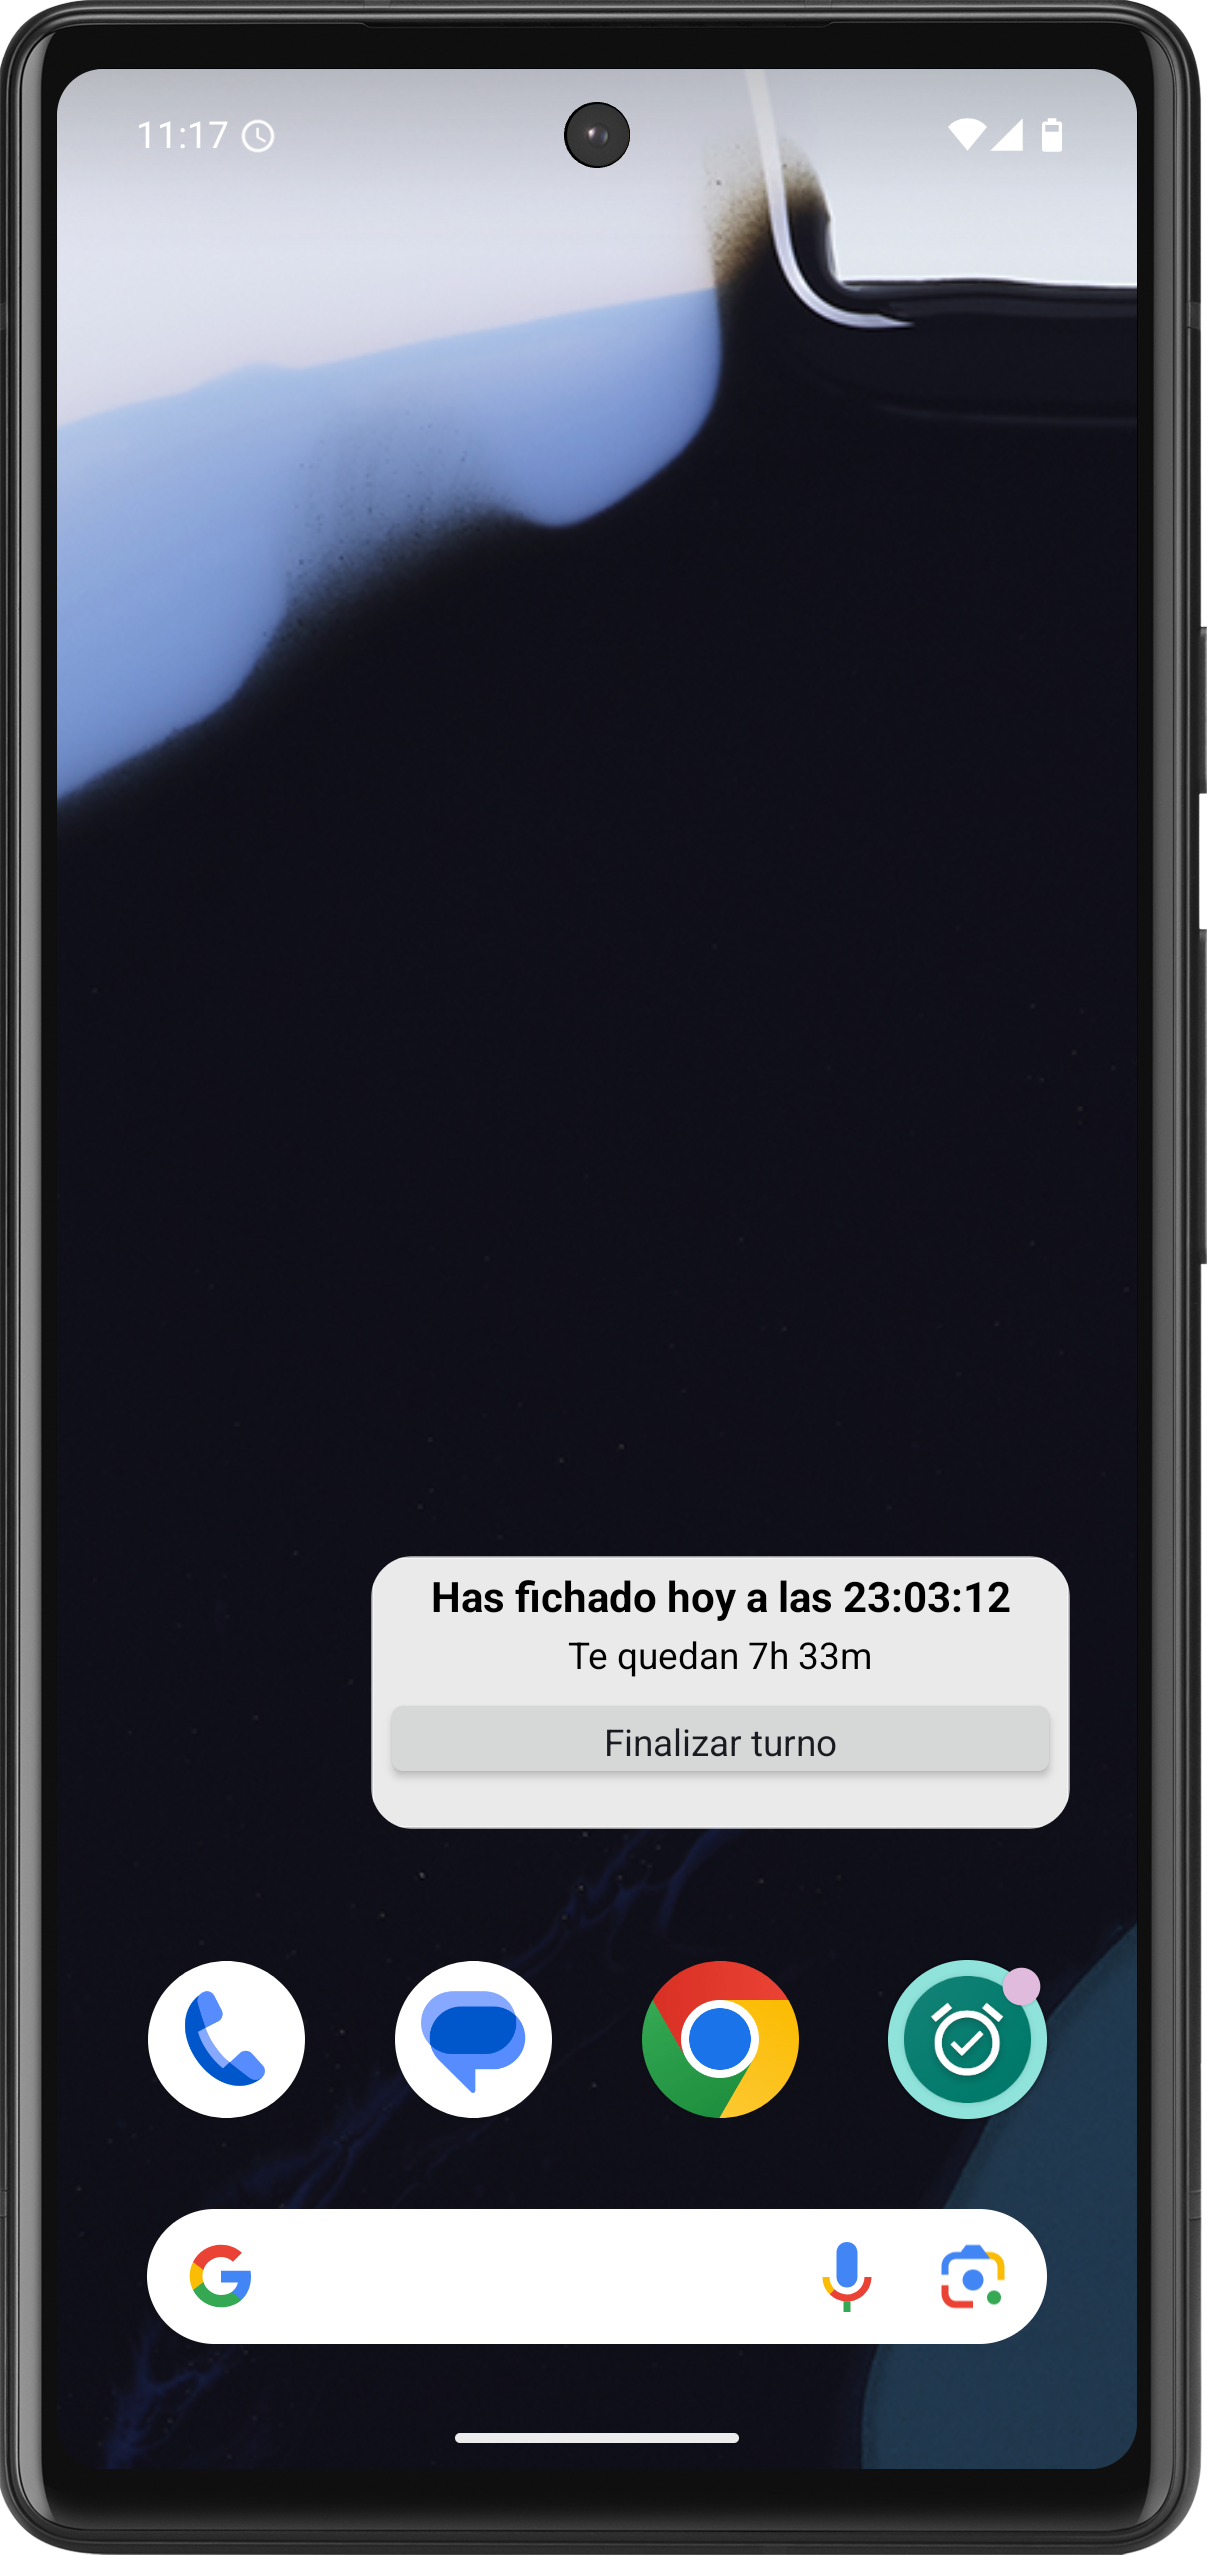
\includegraphics[width=\textwidth]{root/widget.png}
         \caption{Widget de la app}
         \label{fig:widget}
     \end{subfigure}
        \caption{Uso general de la aplicación}
        \label{fig:uso}
\end{figure}

\subsection{Gestión de perfiles}

Con el fin de dar una mejor experiencia de uso, es posible modificar el perfil de usuario. Desde el menú lateral, presionando sobre el icono de la parte superior derecha, es posible acceder a la configuración del perfil. Como se aprecia en la Figura \ref{fig:perfil}, puede establecerse el nombre, los apellidos, el correo electrónico (debe seguir la estructura \textit{nombre@dominio.extension} para que se reconoza como correcto) y la fecha de nacimiento (debe ser superior a los 18 años), así como asignar una foto de perfil, que puede hacerse directamente desde la app o elegirse desde el propio dispositivo. Deben completarse todos los campos para generar el perfil completo de usuario.

Los datos proporcionados se usarán para mejorar la experiencia de usuario. La imagen de perfil se mostrará en el menú, así como el nombre elegido, tal y como representa la Figura \ref{fig:menu}. Puede combinarse con las opciones de la sección de ajustes para conseguir una mayor personalización.

Desde esta misma sección, existe también la opción de cambiar la contraseña, siendo necesario introducir la contraseña actual del usuario y dos veces la nueva contraseña. En cualquier caso, la contraseña debe tener más de 4 caracteres para que se considere válida. También se permite cerrar sesión.

\begin{figure}[H]
     \centering
     \begin{subfigure}[b]{0.4\textwidth}
         \centering
         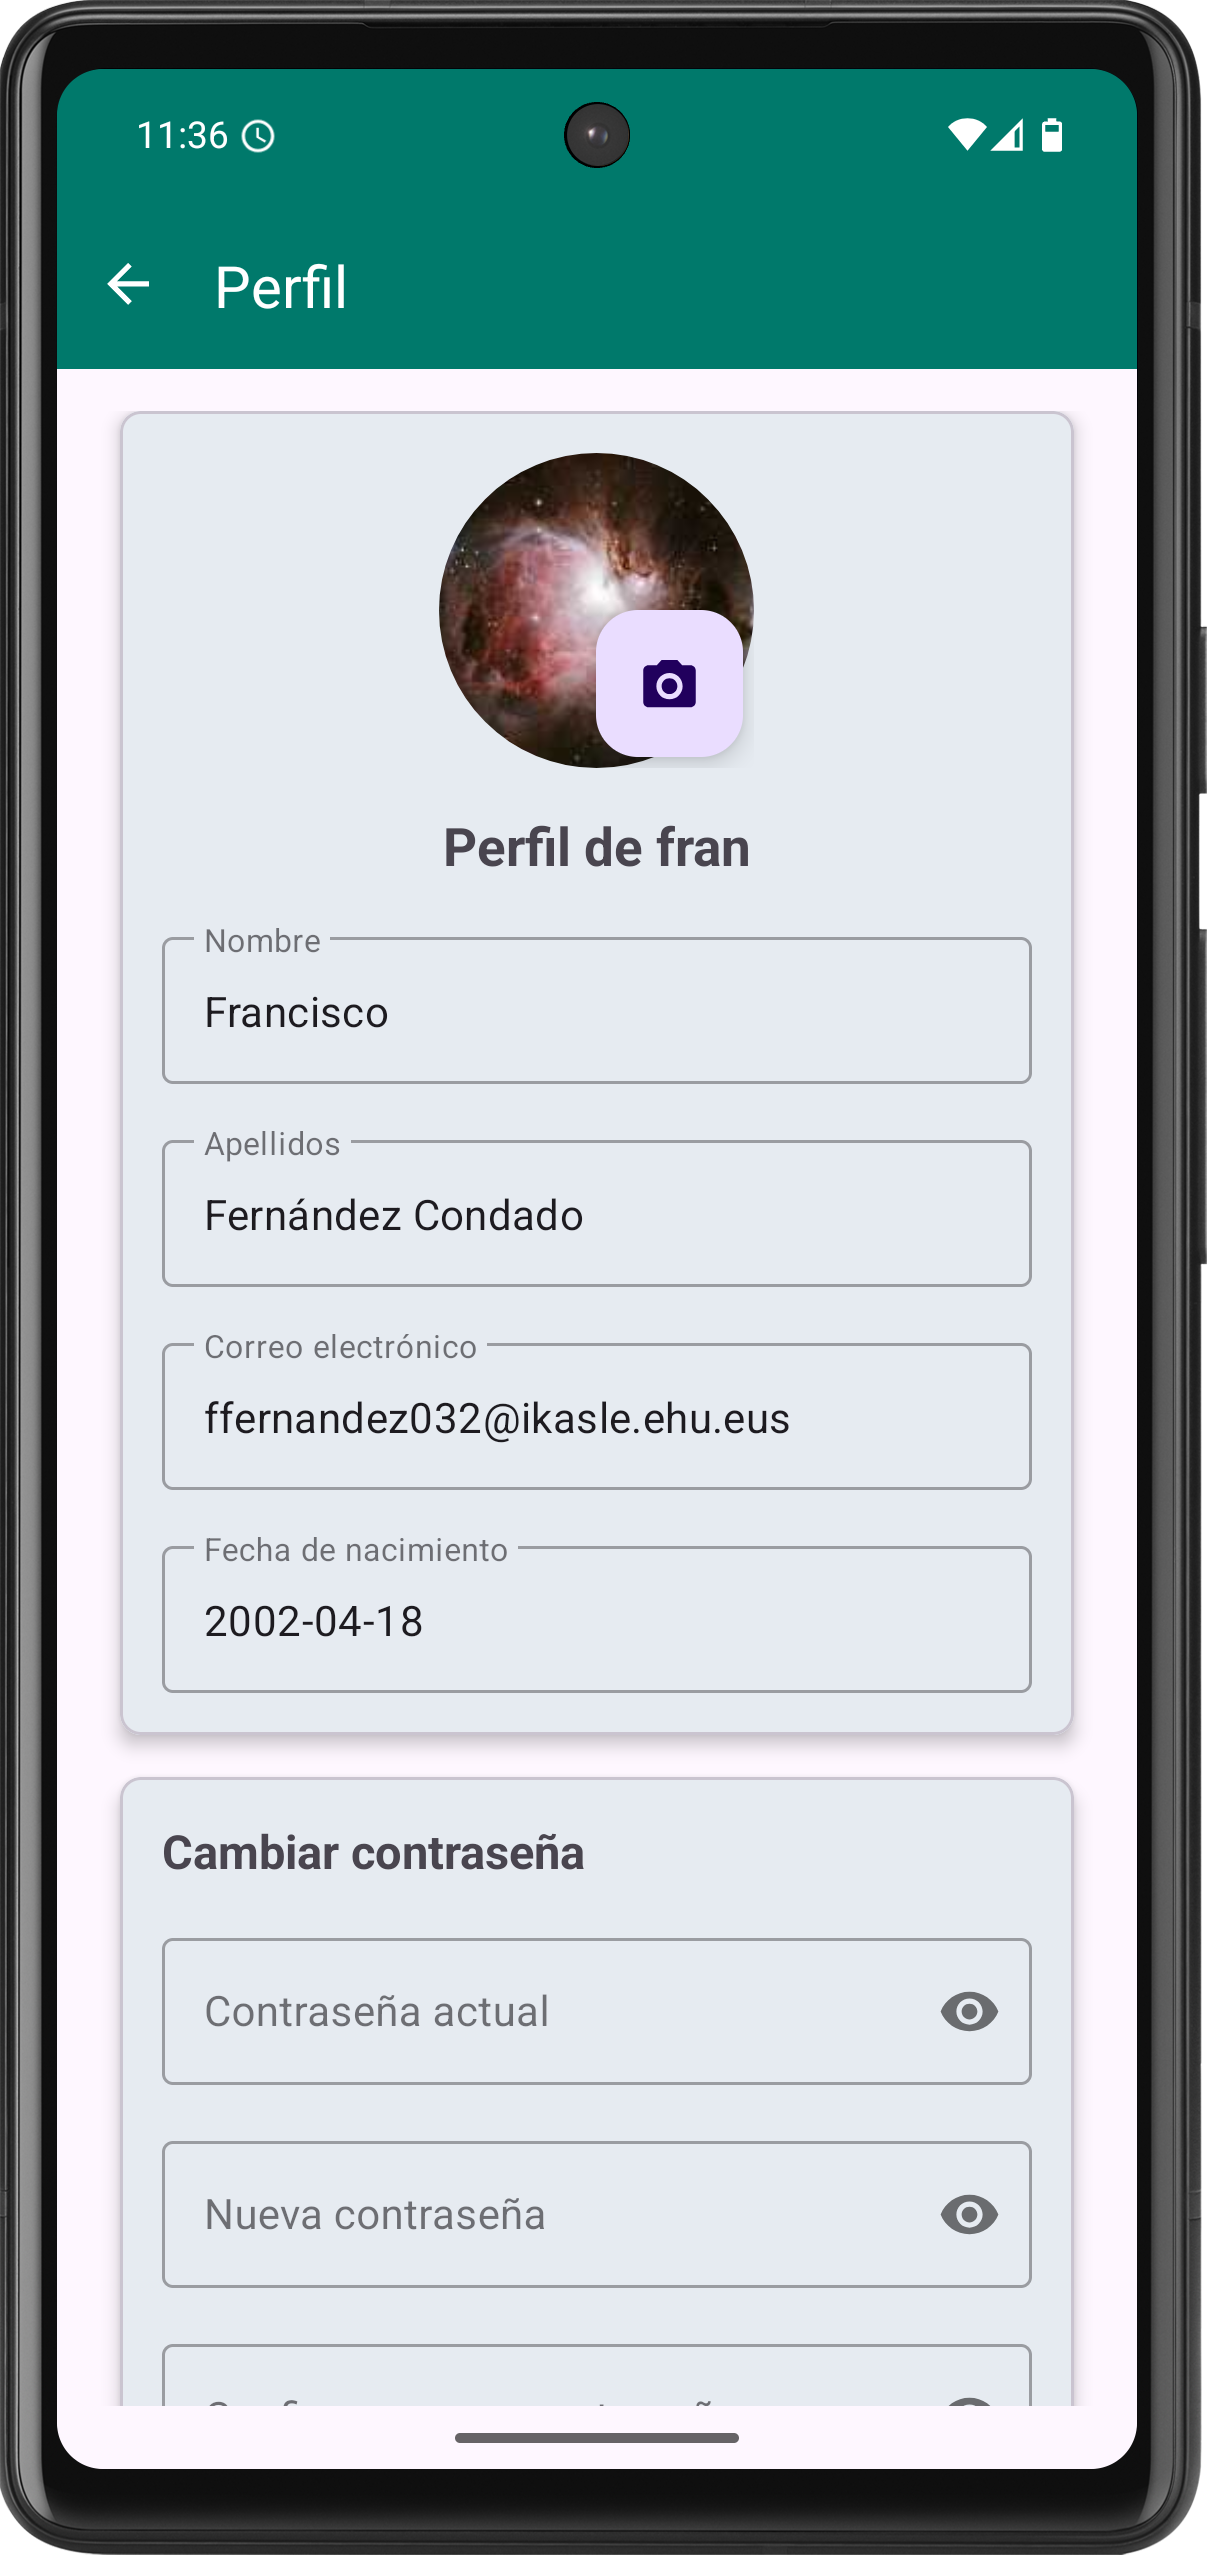
\includegraphics[width=\textwidth]{root/perfil.png}
         \caption{Perfil de usuario}
         \label{fig:perfil}
     \end{subfigure}
     \hfill
     \begin{subfigure}[b]{0.4\textwidth}
         \centering
         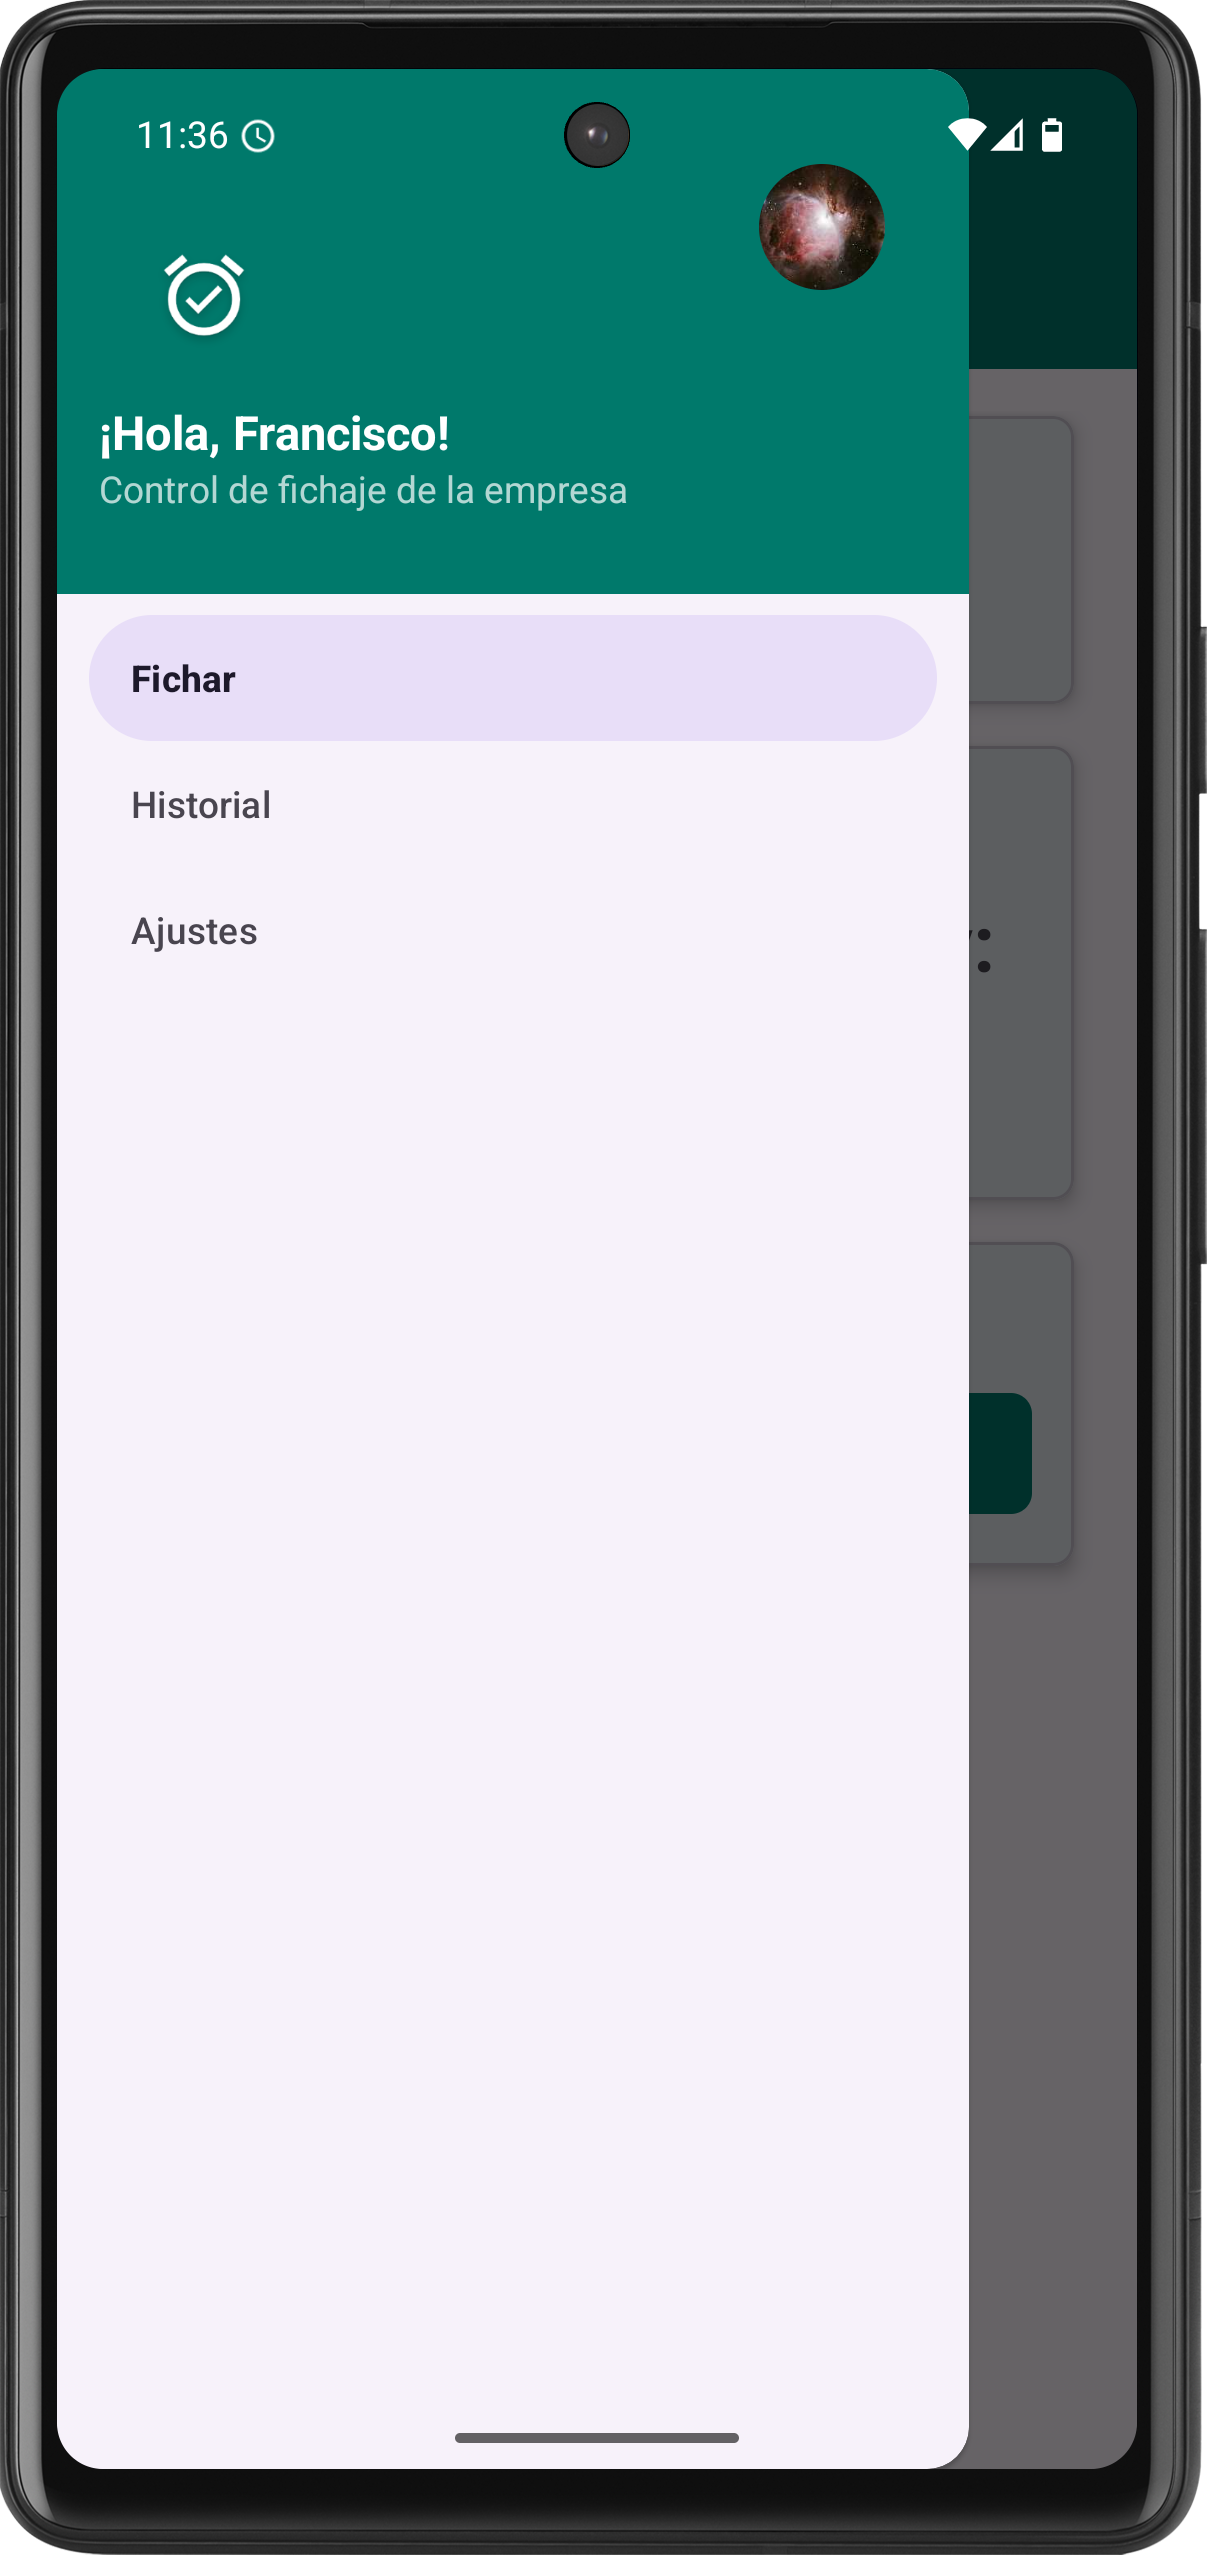
\includegraphics[width=\textwidth]{root/menu.png}
         \caption{Menú de la aplicación}
         \label{fig:menu}
     \end{subfigure}
        \caption{Opciones de personalización de perfil de la aplicación}
        \label{fig:perfiles}
\end{figure}


\section{Dificultades encontradas al realizar el proyecto} \label{ch5}
A lo largo del proyecto, han surgido múltiples dificultades. En primer lugar, el rendimiento de Android Studio y del emulador no es el esperado, lo que ha dificultado algo la tarea. Además, tuve problemas a la hora de gestionar los permisos y cómo se realizaba el conteo del tiempo, pues había que pulsar varias veces para que se registrase una entrada o una salida, y las notificaciones no siempre se enviaban o, peor aún, se enviaban cada segundo obligando a detener la aplicación, algo que fue corregido.

También ha resultado algo complicado implementar la lógica del inicio de sesión, principalmente porque la aplicación se creó siendo pensada para un solo usuario y, por tanto, ha sido necesario adaptar cada método para que funcione correctamente con múltiples usuarios, siendo necesario acceder y añadir un parámetro más en cada consulta. Tampoco ha sido sencillo almacenar las imágenes de perfil en el servidor debido a las limitaciones del mismo, aunque se ha solventado comprimiendo las imágenes y reduciendo su tamaño.

Además, ha resultado algo complicado gestionar el salto de una alarma programada a una hora exacta, principalmente por los permisos y porque en ocasiones se borran. El uso de FCM tampoco ha sido sencillo al haber modificado Google los métodos de acceso para Firebase, requiriendo usar su nueva autenticación. Por último, el \textit{content provider} del calendario tampoco ha sido fácil, debido a que es necesario acceder a las Cuentas para verificar que puede editarse un calendario para añadir un evento.

\section{Fuentes y referencias utilizadas} \label{ch6}
A la hora de realizar el proyecto, ha sido preciso realizar consultas a diferentes sitios de Internet, bien para resolver dudas o para obtener información y guías sobre cómo realizar diferentes acciones. A continuación se exponen las fuentes y referencias más relevantes que se han utilizado:

\begin{itemize}
    \item Apuntes de la asignatura “Desarrollo Avanzado de Software”. Iker Sobrón Polancos. eGela UPV/EHU.
    \item \href{https://developer.android.com/}{Android Developers Guide}.
    \item \href{https://firebase.google.com/docs/cloud-messaging/auth-server}{Firebase Documentation}.
    \item \href{https://www.w3schools.com/js/js_json_php.asp}{JSON PHP. W3Schools}.
    \item \href{https://github.com/osmdroid/osmdroid}{OSMdroid}.
    \item \href{https://github.com/luciferous/jwt}{jwt}.
    \item \href{https://github.com/firebase/php-jwt}{php-jwt}.
    \item \href{https://getbootstrap.com}{Bootstrap}.
    \item \href{https://stackoverflow.com/questions/16616458/how-to-use-resource-arrays-using-xml-in-android}{\textit{Android Studio mensaje: Missing Constraints in ConstraintLayout}. Stack Overflow}.
    \item \href{https://romannurik.github.io/AndroidAssetStudio/icons-launcher.html}{Launcher icon generator}.
    \item \href{https://materialui.co/colors}{Material design color palette}.
\end{itemize}

\label{EndOfText}

% --- Nomenclaturas ---
%\newpage
%\addcontentsline{toc}{section}{Nomenclature}
%\input{sources/9_nomenclat.tex}

% --- Referencias y bibliografía ---
%\newpage
%\addcontentsline{toc}{section}{Referencias}
%\bibliography{document.bib} 
%\bibliographystyle{ieeetr}

% --- Apéndices ---
%\newpage
%\section{Appendix A} \label{ch6}

\label{endOfDoc}
\end{document}
